% ============================================================
% IE UNIVERSITY - BACHELOR IN APPLIED MATHEMATICS
% FIELD - FINAL REPORT (Machine Learning & Communication Skills)
% Built on the official BAM Project LaTeX Template (bam-project.cls, downloaded
% from the course Overleaf project on 18 November 2026; unchanged).
%
% Assignment brief (project_ML_commskills_2026.pdf) requirements kept here:
% - Layout: clean, twocolumn (brief, Section 4: "Select clean,twocolumn").
% - 10-12 pages, excluding the bibliography and appendices.
% - Background integrated into the Introduction; results discussed where shown.
% - References in MLA style (the brief overrides the template's amsplain).
% - Link to the public GitHub repository.
% - Declaration of Contributions as in the template.
%
% HOW TO WRITE: see WRITING_GUIDE.md in this folder. Each member writes only
% the files assigned to them in sections/. Blue boxes (\guide) and grey boxes
% (\budget) are notes for the writer: delete them when the paragraph is written.
% Before submission, set \FIELDdraftfalse below: if any \guide, \budget or
% \capguide is left, compilation stops and names it.
% ============================================================
\documentclass[clean,twocolumn]{bam-project}

% ------------------------------------------------------------
% PROJECT METADATA
% ------------------------------------------------------------
\BAMtitle{FIELD: How Much Does the Field of Study Shape University GPA Rankings?}
\BAMshorttitle{FIELD: field of study and GPA rankings}
\BAMcourse{Machine Learning \& Communication Skills}
\BAMteam{Adam Bajer\\[0.2em]Pablo Torres\\[0.2em]Ignacio Gimeno}
\BAMinstructors{Idris Kouadri Boudjelthia\\[0.2em]Irene Alda Ferrero}
\BAMsubmissiondate{30 November 2026}

% Optional table of contents: not needed in a paper-style report.
\newif\ifBAMshowtoc
\BAMshowtocfalse

% Figures live in the repository's figures/final/ folder.
\graphicspath{{./}{../../figures/final/}}

% ------------------------------------------------------------
% DRAFTING AIDS (remove nothing here; switch the flag before submitting)
% ------------------------------------------------------------
\newif\ifFIELDdraft
\FIELDdrafttrue   % <-- set to \FIELDdraftfalse for the submitted version

% Colours of the overview diagram (same palette as the figures).
\usetikzlibrary{arrows.meta}
\definecolor{FIELDdata}{HTML}{0072B2}
\definecolor{FIELDstep}{HTML}{E69F00}

\definecolor{FIELDguide}{HTML}{1F4E9C}
\newtcolorbox{FIELDguidebox}[1]{%
  enhanced, breakable, colback=FIELDguide!5, colframe=FIELDguide, boxrule=0.5pt,
  arc=1pt, left=4pt, right=4pt, top=3pt, bottom=3pt, before skip=4pt, after skip=5pt,
  fontupper=\footnotesize, title={#1}, fonttitle=\footnotesize\bfseries,
  colbacktitle=FIELDguide, coltitle=white, toptitle=1pt, bottomtitle=1pt}

% \guide{Writer -- paragraph}{what the paragraph must establish, numbers, sources}
\newcommand{\guide}[2]{%
  \ifFIELDdraft
    \begin{FIELDguidebox}{#1}#2\end{FIELDguidebox}%
  \else
    \PackageError{FIELD}{A writing guide is still in the text: #1}%
      {Write the paragraph and delete its \string\guide\space block.}%
  \fi}

% \budget{words}{writer}: grey box with the height of that many words in one
% column, so the draft shows the planned length of the finished report.
\newcommand{\budget}[2]{%
  \ifFIELDdraft
    \par\noindent{\color{black!35}\fboxsep=0pt\fbox{\parbox[c][\dimexpr\textheight*#1/600\relax][c]{\dimexpr\linewidth-2\fboxrule\relax}{%
      \centering\footnotesize\color{black!55}about #1 words of text (#2)}}}\par
  \else
    \PackageError{FIELD}{A length placeholder is still in the text (#2, #1 words)}%
      {Delete the \string\budget\space line once the text is written.}%
  \fi}

% \capguide{...} inside \caption: what the caption must state.
\DeclareRobustCommand{\capguide}[1]{%
  \ifFIELDdraft
    {\color{FIELDguide}[Caption to write: #1]}%
  \else
    \PackageError{FIELD}{A caption is still a placeholder}{Write the caption.}%
  \fi}

% MLA in-text citations are written by hand, e.g. (Achen and Courant 80).
% Works Cited is in sections/90_works_cited.tex.

\begin{document}

\makebamtitle

% ============================================================
% ABSTRACT
% ============================================================
\begin{BAMabstract}
% ============================================================
% ABSTRACT -- Writer: Ignacio Gimeno
% Every number appears in Section 4. Recheck after Adam's and Pablo's sections
% are merged (US result and selection numbers).
% ============================================================

Universities often rank students from different degrees on a single grade point average (GPA) list to allocate exchange places, grants or admission to master's programmes, which assumes that a grade means the same in every field. We ask how much of a student's position in such a ranking depends on their field of study, and how ranking students within their degree would change who is selected. We analyse three separate datasets: 12,125 mean graduate grades from 89 Spanish universities (2015--16 to 2023--24), the records of 3,703 Portuguese students and course grades from 33 US public universities. Within Spanish universities, 65\% of the variation in grades between fields is a field effect shared by all universities and 28\% is specific to each university. In a supervised regression task with five models tuned on 2018--2021 and tested once on 2022--2023, our main model, a shrunk profile of each university's past deviations, reduces the prediction error from 0.225 to 0.138 grade points relative to the shared field effect; gradient boosting improves on it only slightly (0.133). In a simulated top-20\% selection, 41\% of Nursing graduates are selected against 6\% of Business administration graduates. Subtracting each university's past field deviation from the marks lowers the average distance from equal access from 11.8 to 5.1 percentage points, but cannot remove differences in the spread of grades. Ranking students within their degree reduces the spread of selection rates across degrees from 0.090 to 0.006, while the next-semester grade of those selected changes only from 14.21 to 14.08 out of 20. A single raw-GPA ranking therefore sorts students largely by field, and ranking within the degree corrects this at almost no cost.

\BAMkeywords{grade comparability; GPA ranking; field of study; mixed-effects models; temporal validation; fair selection}

\end{BAMabstract}

% ============================================================
% 1. INTRODUCTION (background and related work integrated, as the brief requires)
% ============================================================
\section{Introduction}
\label{sec:introduction}
% ============================================================
% 1.1 INTRODUCTION: STUDENTS' BACKGROUNDS -- Writer: Ignacio Gimeno
% Target: about 280 words + Figure 1 (student background by degree). The Introduction is split in three files: 01a (Ignacio), 01b (Adam), 01c (Ignacio).
% Brief: "Introduction, including Background and Related Work: research
% question, motivation, dataset significance, objectives, and the relevant
% scientific or technical background and prior work ... integrated into the
% Introduction rather than submitted as a separate chapter."
% IRENE'S FEEDBACK ON THE SENTENCE OUTLINE (follow it in this order):
%   "Begin with how students' backgrounds can shape their choice of degree,
%    then explain why GPA comparisons across fields raise a fairness question."
%   "expand the literature beyond the current five references"
%   "use graphs to help readers understand the analysis ... interpret the visuals"
%   "Use first-person plural consistently to describe your work"
% Template: avoid a broad textbook opening; every objective must connect to a
% result and a conclusion; signpost the report without listing section titles.
% All references below were checked (Crossref) and are in 90_works_cited.tex.
% ============================================================

\subsection{Students' Backgrounds and the Choice of Degree}
\label{sec:context}

\guide{Ignacio -- Paragraph 1: background shapes the choice of degree (literature)}{%
\textbf{Establish (Irene):} the degree a student enters is not random: family background, gender, preferences and prior achievement shape it.\\
\textbf{Sources (MLA in-text):} family socioeconomic status and parental involvement are linked to the choice of major, with differences by gender, ethnicity and nativity (Ma); the gender gap in majors is explained mainly by preferences and tastes rather than by expected ability (Zafar); students sort into majors by ability (Arcidiacono); review of how school curriculum and major choice differ across students and shape careers (Altonji et al.). Compare them in two or three sentences; do not list them.}
\budget{140}{Ignacio}

\guide{Ignacio -- Paragraph 2: our own data show it (Figure~\ref{fig:background})}{%
\textbf{Interpret the figure (Irene: interpret the visuals):} in the 3,703 Portuguese students, the share with at least one parent holding a higher-education degree ranges from 7\% (Social Service, evening) to 50\% (Equinculture), scholarship holders from 8\% (Equinculture) to 42\% (Social Service), women from 2\% (Informatics Engineering) to 95\% (Basic Education); all differences between degrees are far larger than chance ($\chi^2$ tests, 14 df, $p<10^{-25}$; entry grade ANOVA $F = 12.6$, $p < 10^{-28}$). Across the 15 degrees, mean GPA is higher where more students have a graduate parent ($r = 0.40$) and stronger entry grades ($r = 0.44$).\\
\textbf{Why it matters for the question:} degrees differ in who enters them, so a pooled GPA ranking compares students from different backgrounds \emph{and} different grading practices -- the report separates the second from the first as far as the data allow (\S\ref{sec:res-confounders}).\\
\textbf{Source:} \texttt{results/background\_stats.json}, \texttt{results/background\_by\_degree.csv}. Descriptive only: no causal claim.}
\budget{140}{Ignacio}

\begin{figure*}[t]
  \centering
  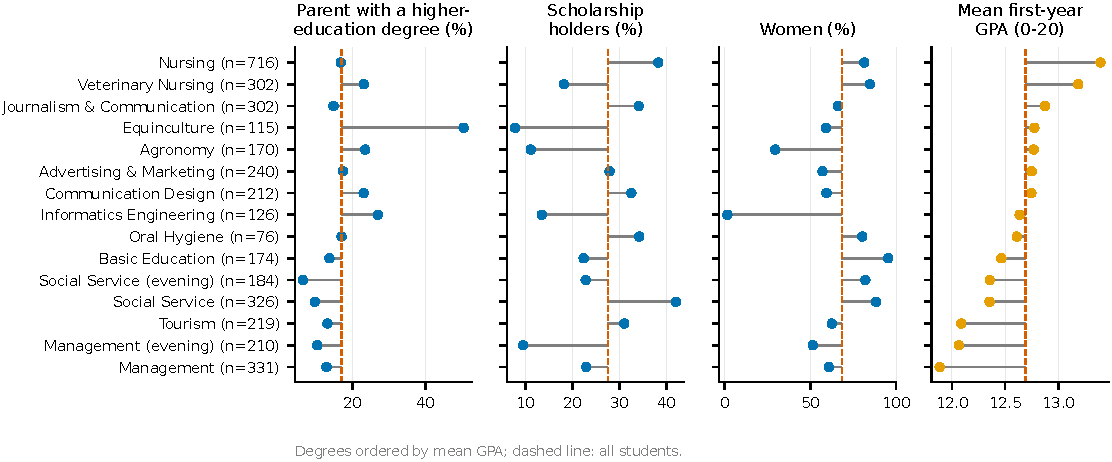
\includegraphics[width=\textwidth]{fig9_background}
  \caption{\capguide{Ignacio -- what is shown (background of the students of each degree, 15 degrees, 3,703 students of one Portuguese polytechnic, cohorts 2008--09 to 2018--19); definition of ``parent with a higher-education degree'' (mother or father with a completed bachelor's, master's or doctorate); degrees ordered by mean first-year GPA; dashed line = all students; source (Realinho et al.).}}
  \label{fig:background}
\end{figure*}


% ============================================================
% 1.2 INTRODUCTION: THE FAIRNESS QUESTION -- Writer: Adam Bajer
% Target: about 300 words. Comes right after Ignacio's 1.1 (backgrounds and Figure 1); read it first so the two parts connect.
% Brief: "Introduction, including Background and Related Work: research
% question, motivation, dataset significance, objectives, and the relevant
% scientific or technical background and prior work ... integrated into the
% Introduction rather than submitted as a separate chapter."
% IRENE'S FEEDBACK ON THE SENTENCE OUTLINE (follow it in this order):
%   "Begin with how students' backgrounds can shape their choice of degree,
%    then explain why GPA comparisons across fields raise a fairness question."
%   "expand the literature beyond the current five references"
%   "use graphs to help readers understand the analysis ... interpret the visuals"
%   "Use first-person plural consistently to describe your work"
% Template: avoid a broad textbook opening; every objective must connect to a
% result and a conclusion; signpost the report without listing section titles.
% All references below were checked (Crossref) and are in 90_works_cited.tex.
% ============================================================

\subsection{Why Comparing GPAs Across Fields Raises a Fairness Question}
\label{sec:fairness}

\guide{Adam -- Paragraph 1 of 1.2: fields grade differently, and grades steer choices}{%
\textbf{Establish:} departments grade differently (Achen and Courant; Sabot and Wakeman-Linn), across many universities (Jeong et al.); low grades push students out of science majors (Ost; Rask) and students move towards leniently graded courses when grade information is visible (Bar et al.; read its abstract first); when Wellesley capped average grades in high-grading departments, enrolment in those departments fell (Butcher et al.). So grading practices and choices feed each other.}
\budget{140}{Adam}

\guide{Adam -- Paragraph 2 of 1.2: the fairness question}{%
\textbf{Establish (Irene):} universities and programmes rank students from different degrees on one GPA list (exchange places, grants, honours, master's admission); if a grade does not mean the same in every field, the list partly sorts students by the field they chose -- and, through \S\ref{sec:context}, by their background. One concrete example the reader knows (exchange-place allocation).\\
\textbf{Existing answers:} adjusted GPAs that model each course's grading (Young; Johnson); comparisons of GPA measures against later outcomes (Bailey et al. -- read the abstract first); grade distribution tables to compare grades across groups (European Commission, ECTS Users' Guide).\\
\textbf{Make clear (outline 2a):} we measure differences in \emph{observed grades}; we do not claim a field is harder or its students better.\\
\textbf{Idris's feedback:} announce that we test his adjusted mark (original mark minus the field deviation) on selection outcomes.}
\budget{160}{Adam}


% ============================================================
% 1.3 INTRODUCTION: QUESTION AND OBJECTIVES -- Writer: Ignacio Gimeno
% Target: about 230 words.
% Brief: "Introduction, including Background and Related Work: research
% question, motivation, dataset significance, objectives, and the relevant
% scientific or technical background and prior work ... integrated into the
% Introduction rather than submitted as a separate chapter."
% IRENE'S FEEDBACK ON THE SENTENCE OUTLINE (follow it in this order):
%   "Begin with how students' backgrounds can shape their choice of degree,
%    then explain why GPA comparisons across fields raise a fairness question."
%   "expand the literature beyond the current five references"
%   "use graphs to help readers understand the analysis ... interpret the visuals"
%   "Use first-person plural consistently to describe your work"
% Template: avoid a broad textbook opening; every objective must connect to a
% result and a conclusion; signpost the report without listing section titles.
% All references below were checked (Crossref) and are in 90_works_cited.tex.
% ============================================================

\subsection{Research Question, Objectives and Contribution}
\label{sec:objectives}

\guide{Ignacio -- Paragraph 3 of the Introduction: question, objectives and gap}{%
\textbf{Research question (identical to the README):} how much of a student's position in a university-wide GPA ranking depends on their field of study, and how would ranking students within their degree change who is selected for a fixed number of places?\\
\textbf{Gap, stated modestly:} most studies use one university or US data; we (i) separate a field effect shared by 89 Spanish universities from each university's own pattern, (ii) test with tuned machine-learning models whether these patterns predict unseen years, and (iii) judge corrections by what they do to selection and to later performance.\\
\textbf{Objectives, each pointing to its answer:} O1 field effects, shared and university-specific (\S\ref{sec:res-field}); O2 persistence and prediction (\S\ref{sec:res-prediction}); O3 does intake explain them (\S\ref{sec:res-confounders}); O4 consequence for a top-20\% selection (\S\ref{sec:res-selection}); O5 the adjusted mark and within-degree ranking (\S\ref{sec:res-adjusted}, \S\ref{sec:res-rules}); O6 the US check (\S\ref{sec:res-us}).}
\budget{160}{Ignacio}

\guide{Ignacio -- Paragraph 4 of the Introduction: scope and road map}{%
Three separate datasets that cannot be linked; aggregated means in Spain, so associations, not causes (\S\ref{sec:res-limitations}). Two or three sentences telling the reader what each part shows (Figure~\ref{fig:overview} gives the map of the analysis), not a list of section titles.}
\budget{70}{Ignacio}



% ============================================================
% 2. DATA
% ============================================================
\section{Data}
\label{sec:data}
% ============================================================
% 2. DATA -- Writer: Pablo Torres (2.1, 2.2, overview) and Adam Bajer (2.3, in
% 02b_data_us.tex). Target: about 480 words for Pablo, 170 for Adam, + Table 1.
% Brief: "Data, Materials, or Inputs: sources, provenance, integration,
% preparation, limitations, and any relevant ethical or access considerations."
% Template: source and access conditions; sampling; inclusion and exclusion
% criteria; units and variable definitions; cleaning; missing values; licensing;
% privacy or ethics; known limitations.
% IMPORTANT (Idris, Progress Report feedback): the data was hard to understand.
% This section must make the unit of observation of each dataset obvious.
% Start from outline entries 3, 3a, 3b, 3c.
% ============================================================

\guide{Pablo -- Overview paragraph + Table~\ref{tab:data}}{%
\textbf{Establish (outline 3):} three datasets are analysed separately because they have different units of observation and cannot be linked; one sentence on what each contributes.\\
\textbf{Introduce Table~\ref{tab:data}} in the text and tell the reader what to look at in it (the unit of observation row). Write the table caption yourself (the blue text in the caption).}
\budget{80}{Pablo}

% Table 1 -- the three datasets. Numbers checked against results/ on 20 Nov 2026:
% summary_stats.json (Portugal 3,703 students, 15 degrees), ranking_rules.json
% (3,469 students), progress_stats.json (match: 86 with dropout, 47 with admission),
% normal_check_stats.json (10,476 matched records, 664 university-years, 79
% universities), us_replication_stats.json (1,449,779 raw rows; 1,845 cells;
% 29 weighted universities; 2009-2023), mixed_model_stats.json (12,125; 89; 29).
\begin{table*}[t]
\centering
\caption{Coverage and units of observation of the three separately analysed datasets; analysis sample sizes are after preparation, with original sizes identified where relevant. SIIU denotes the Sistema Integrado de Informaci\'on Universitaria; IQR denotes interquartile range. Sources: Ministry tables, Realinho et al.\ and Jeong et al.; sample counts from the saved results.}
\label{tab:data}
\small
\begin{tabularx}{\textwidth}{@{}l>{\raggedright\arraybackslash}X>{\raggedright\arraybackslash}X>{\raggedright\arraybackslash}X@{}}
\toprule
 & Spain (Ministry, SIIU) & Portugal (UCI records) & United States (33 universities) \\
\midrule
Unit of observation & Mean final grade of the graduates of one field at one university in one academic year (with quartiles and maximum) & One student (first-year grades by semester, entry grade, degree) & One course or section (share of each letter grade, enrolment) \\
Size used & 12,125 university-field-years; 89 universities; 29 fields & 3,703 students in 15 degrees (of 4,424); 3,469 with grades in both semesters & 1,449,779 rows; 1,845 university-area-year cells; 10 broad areas \\
Period & 2015--16 to 2023--24 & cohorts 2008--09 to 2018--19 & 2009 to 2023 (source years) \\
Grade scale & 5--10 & 0--20 & 0--4 (A+ = 4.3) \\
Extra variables & dropout (86 universities), graduates per field, admission grade by broad branch (47 public universities) & admission grade, standardised within admission route; background variables & enrolment (missing at 4 institutions) \\
Used for & field effects, prediction, selection simulation, adjusted marks & degree gap with entry grades, ranking rules & external check of broad-area effects \\
Source & Ministerio de Ciencia, Innovaci\'on y Universidades & Realinho et al. & Jeong et al. \\
\bottomrule
\end{tabularx}
\end{table*}


\subsection{Spanish Ministry Data}
\label{sec:data-spain}

\guide{Pablo -- Paragraph: what one observation is}{%
\textbf{Establish (outline 3a):} one row = mean final grade (\emph{nota media del expediente}) of the graduates of one field at one university in one academic year; the Ministry also publishes the quartiles and the maximum. 12,125 rows, 89 universities, 29 fields (\emph{\'ambitos de estudio}), 2015--16 to 2023--24, scale 5--10, both sexes combined.\\
\textbf{Missing cells:} the Ministry hides small cells, so only about half of the possible university-field-years appear (12,125 of $89\times29\times9=23{,}229$, i.e.\ 52\%); models use reported cells only.\\
\textbf{Cite:} Ministerio de Ciencia, Innovaci\'on y Universidades, ``Media, cuartiles y m\'aximo\ldots'' (see Works Cited).}
\budget{130}{Pablo}

\guide{Pablo -- Paragraph: extra Ministry tables and how they are matched}{%
\textbf{Variables:} dropout rate by university and field (86 universities); number of graduates by university, field and year (weights and size); admission grade of new entrants, published only by university and \emph{broad branch} (5 branches for 29 fields) and only for 47 public universities; national admission grade by field.\\
\textbf{Preparation:} admission grades converted to $z$-scores because branch scales differ; graduates matched to grades by university, field and year (10,476 records with valid quartiles and counts are used in the selection simulation).\\
\textbf{Limitation to state here:} the admission grade cannot separate fields within one branch (keep the full discussion for \S\ref{sec:res-confounders}).}
\budget{110}{Pablo}

\subsection{Portuguese Student Records}
\label{sec:data-portugal}

\guide{Pablo -- Paragraph: individual students}{%
\textbf{Establish (outline 3b):} 4,424 students of one Portuguese polytechnic, enrolled 2008--09 to 2018--19 (Realinho et al.); first-year GPA = mean of the two semester averages weighted by units passed (scale 0--20).\\
\textbf{Cleaning (src/load\_data.py):} students who passed no unit are excluded because their average is undefined, not zero; degrees with fewer than 50 students are excluded; result 3,703 students in 15 degrees. The ranking-rule comparison uses the 3,469 students with grades in both semesters.\\
\textbf{Entry grades:} standardised within admission route because routes grade applicants differently.\\
\textbf{Why this dataset matters:} it is the only one with individual students and entry grades, so it can test corrections on later performance.\\
\textbf{Access and ethics:} public, anonymised data (UCI Machine Learning Repository, Creative Commons Attribution 4.0 licence, checked on the dataset page on 22 Nov 2026). The same records give the background variables of Figure~\ref{fig:background} (parents' qualifications, scholarship, gender).}
\budget{160}{Pablo}

% ============================================================
% 2.3 US COURSE GRADES -- Writer: Adam Bajer -- about 170 words
% Start from outline entry 3c. Numbers: results/us_replication_stats.json,
% README "US replication (Adam)".
% ============================================================

\subsection{US Course Grades}
\label{sec:data-us}

\guide{Adam -- Paragraph: what one observation is and how it was prepared}{%
\textbf{Establish (outline 3c):} grade distributions at the course or section level from 33 US public universities (Jeong et al.; dataset ``Course Grades from 33 Public Universities'' on Kaggle, MIT licence). One row = share of each letter grade in one course or section, with total enrolment; these are \emph{not} individual students' GPAs.\\
\textbf{Preparation:} section GPA from the letter shares with the paper's mapping (A+ = 4.3 \ldots\ F = 0; pass/fail and withdrawals excluded); 1,449,779 raw rows, 94\% of valid rows mapped to a broad area; exact duplicates removed; four institutions without enrolment counts are excluded from the weighted analysis (Georgia Tech, Parkland College, Purdue, UNC Charlotte).\\
\textbf{Limitation to state here:} source years 2009--2023 do not match the Spanish window.\\
Keep the mapping to ten broad areas for \S\ref{sec:methods-us}.}
\budget{170}{Adam}



% ============================================================
% 3. METHODOLOGY
% ============================================================
\section{Methodology}
\label{sec:methodology}
% Figure: map of the analysis (Irene: "use graphs to help readers understand the
% analysis"). Drawn in TikZ so it uses the report's fonts. Original diagram.
% Introduced by Pablo at the start of Section 3 and referred to in the
% Introduction road map. Numbers checked against results/ on 22 Nov 2026.
\begin{figure*}[t]
\centering
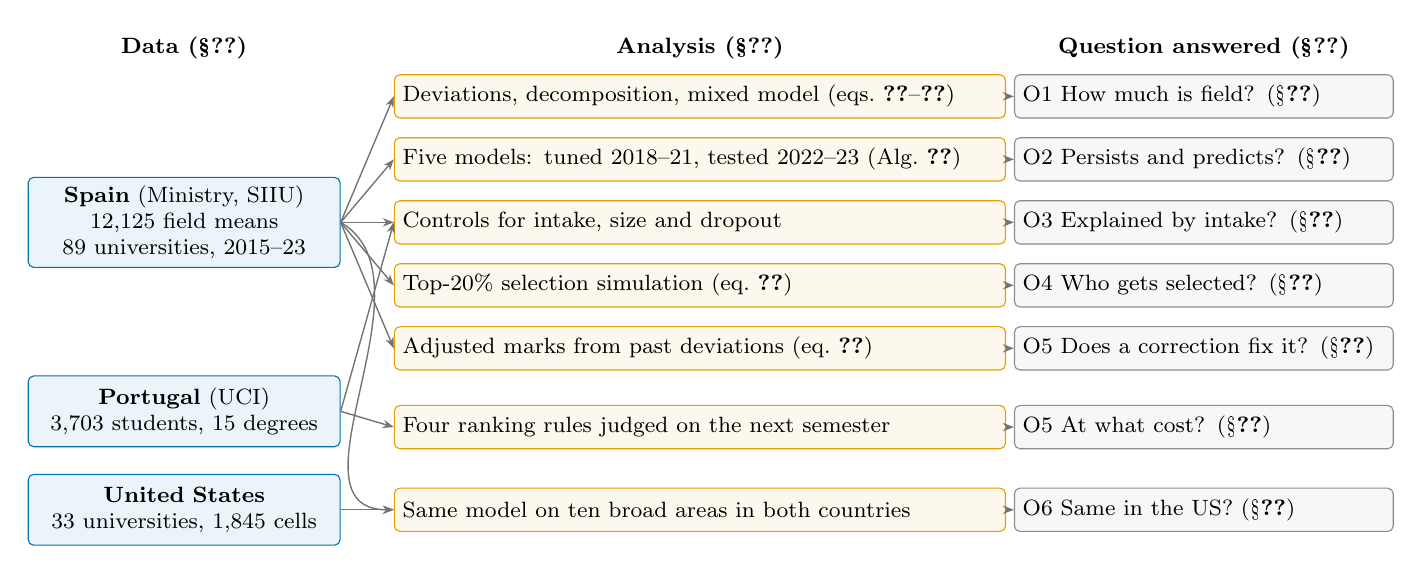
\begin{tikzpicture}[
  font=\footnotesize,
  fdata/.style={draw=FIELDdata, fill=FIELDdata!8, rounded corners=2pt, align=center, text width=3.75cm, minimum height=0.9cm, inner sep=3pt},
  fstep/.style={draw=FIELDstep, fill=FIELDstep!7, rounded corners=2pt, align=left, text width=7.55cm, minimum height=0.55cm, inner sep=3pt},
  fgoal/.style={draw=black!45, fill=black!3, rounded corners=2pt, align=left, text width=4.6cm, minimum height=0.55cm, inner sep=3pt},
  arr/.style={-{Stealth[length=4pt]}, draw=black!55, line width=0.5pt},
  hdr/.style={font=\footnotesize\bfseries, anchor=south}
]
% columns
\node[hdr] at (0,0.35) {Data (\S\ref{sec:data})};
\node[hdr] at (6.55,0.35) {Analysis (\S\ref{sec:methodology})};
\node[hdr] at (12.95,0.35) {Question answered (\S\ref{sec:results})};
% data
\node[fdata] (es) at (0,-1.6) {\textbf{Spain} (Ministry, SIIU)\\12,125 field means\\89 universities, 2015--23};
\node[fdata] (pt) at (0,-4.0) {\textbf{Portugal} (UCI)\\3,703 students, 15 degrees};
\node[fdata] (us) at (0,-5.25) {\textbf{United States}\\33 universities, 1,845 cells};
% steps
\node[fstep] (s1) at (6.55,0)    {Deviations, decomposition, mixed model (eqs.~\ref{eq:deviation}--\ref{eq:mixed})};
\node[fstep] (s2) at (6.55,-0.8) {Five models: tuned 2018--21, tested 2022--23 (Alg.~\ref{alg:tuning})};
\node[fstep] (s3) at (6.55,-1.6) {Controls for intake, size and dropout};
\node[fstep] (s4) at (6.55,-2.4) {Top-20\% selection simulation (eq.~\ref{eq:selection})};
\node[fstep] (s5) at (6.55,-3.2) {Adjusted marks from past deviations (eq.~\ref{eq:adjusted})};
\node[fstep] (s6) at (6.55,-4.2) {Four ranking rules judged on the next semester};
\node[fstep] (s7) at (6.55,-5.25) {Same model on ten broad areas in both countries};
% goals
\node[fgoal] (g1) at (12.95,0)    {O1 How much is field? (\S\ref{sec:res-field})};
\node[fgoal] (g2) at (12.95,-0.8) {O2 Persists and predicts? (\S\ref{sec:res-prediction})};
\node[fgoal] (g3) at (12.95,-1.6) {O3 Explained by intake? (\S\ref{sec:res-confounders})};
\node[fgoal] (g4) at (12.95,-2.4) {O4 Who gets selected? (\S\ref{sec:res-selection})};
\node[fgoal] (g5) at (12.95,-3.2) {O5 Does a correction fix it? (\S\ref{sec:res-adjusted})};
\node[fgoal] (g6) at (12.95,-4.2) {O5 At what cost? (\S\ref{sec:res-rules})};
\node[fgoal] (g7) at (12.95,-5.25) {O6 Same in the US? (\S\ref{sec:res-us})};
% arrows data -> steps
\foreach \s in {s1,s2,s3,s4,s5} \draw[arr] (es.east) -- (\s.west);
\draw[arr] (pt.east) -- (s3.west);
\draw[arr] (pt.east) -- (s6.west);
\draw[arr] (us.east) -- (s7.west);
\draw[arr] (es.east) to[out=-30,in=180] (s7.west);
% arrows steps -> goals
\foreach \i in {1,...,7} \draw[arr] (s\i.east) -- (g\i.west);
\end{tikzpicture}
\caption{Map of our analysis: datasets on the left feed the methods in the centre, which answer the numbered questions and results subsections on the right. We analysed the datasets separately without linking individual records between countries. Arrows show analytical use, not data linkage; displayed sample counts come from the saved results. Original diagram.}
\label{fig:overview}
\end{figure*}

% ============================================================
% 3.1-3.4 METHODOLOGY (core) -- Writer: Pablo Torres
% Target: about 1,000 words + equations (1)-(4).
% Brief: "Methodology or Approach: methods applied, implementation choices, and
% rationale." Template: "Each methodological decision should have a reason.
% Separate established methods from modifications or original decisions made by
% the team." Introduce every equation in the text and explain every symbol and
% unit. Results do NOT go here (they go in Section 4).
% The equations below follow the code exactly (src/progress.py, mixed_model.py,
% ministry.py, normal_check.py, final_figures.py). Keep the notation, explain
% it in your own words, and change it only together with Ignacio and Adam so
% that the whole report uses the same symbols.
% Start from outline entries 4, 4a, 4b, 4c, 5, 5a.
% ============================================================

We organised the analysis around three linked questions: how much grade variation belongs to the field, whether a university's particular field pattern persists, and how those differences affect access to a pooled ranking. Figure~\ref{fig:overview} maps this design. Reading left to right, we move from each dataset to the analysis it supports and then to the question and results subsection where we answer it. The arrows connect analytical tasks, not individual records across countries. We first define deviations and estimate variance components, then examine intake, simulate selection and describe uncertainty before presenting the prediction and ranking procedures in Sections~\ref{sec:methods-prediction}--\ref{sec:methods-computing}.
\subsection{Field Deviations and Variance Decomposition}
\label{sec:methods-decomposition}

We made fields comparable within a university and year by subtracting that university's average across its reported fields. In equation~\eqref{eq:deviation}, $\bar g_{ufy}$ is the mean final grade for university $u$, field $f$ and academic year $y$, measured in grade points on the 5--10 scale. The set $F_{uy}$ contains the fields reported for that university-year, and $|F_{uy}|$ is its size; $f'$ indexes the fields being averaged. The resulting deviation $d_{ufy}$ is positive when the field grades above its university-year average and negative when it grades below. We gave reported fields equal weight here, keeping the decomposition distinct from graduate-weighted selection.
\begin{equation}
  d_{ufy} \;=\; \bar g_{ufy} \;-\; \frac{1}{|F_{uy}|}\sum_{f' \in F_{uy}} \bar g_{uf'y}.
  \label{eq:deviation}
\end{equation}
We fitted nested least-squares models to separate a common field pattern from university-specific differences. In equation~\eqref{eq:decomposition}, $\alpha_{uy}$ captures the university-year level, $\beta_f$ the shared field effect, $\gamma_{uf}$ the additional effect of that field at that university, and $\varepsilon_{ufy}$ the unexplained annual variation. We first included $\alpha_{uy}$, then added $\beta_f$, and finally $\gamma_{uf}$. We measured each contribution by the reduction in residual sum of squares divided by the variation remaining after the university-year effects; the final residual forms the noise share. Thus the percentages describe differences within university-years, not all variation in students' grades. We used an $F$-test to compare models with and without the interaction across 1,528 observed university-field cells. We sum-coded field effects, imposing $\sum_f\beta_f=0$, so an effect measures distance from the average field rather than from a chosen reference subject.
\begin{equation}
  \bar g_{ufy} \;=\; \alpha_{uy} + \beta_f + \gamma_{uf} + \varepsilon_{ufy},
  \qquad \textstyle\sum_f \beta_f = 0.
  \label{eq:decomposition}
\end{equation}
\subsection{Mixed-Effects Model}
\label{sec:methods-mixed}

We complemented this decomposition with the mixed-effects model in equation~\eqref{eq:mixed}, fitted to the same 12,125 aggregate means using statsmodels (Seabold and Perktold). Here $\mu$ is the intercept, $\beta_f$ and $\tau_y$ are fixed field and year effects, $a_u$ is a random university intercept, and $b_{uf}$ is the random effect of a field within a university. We assumed independent, zero-mean normal random effects with variances $\sigma_a^2$ and $\sigma_b^2$, and normal residuals $\varepsilon_{ufy}$ with variance $\sigma^2$; $\mathcal N$ denotes the normal distribution. We estimated these variances by restricted maximum likelihood (REML) using the limited-memory Broyden--Fletcher--Goldfarb--Shanno optimiser (L-BFGS). Partial pooling draws less precisely estimated university profiles towards the shared pattern instead of treating every observed difference as equally reliable. We weighted aggregate means equally. For the descriptive comparison, we combined the spread of fitted fixed field effects with the interaction and residual variances, excluding university intercepts and year effects. This and the nested least-squares split estimate different quantities, so we compared their broad patterns rather than treating their percentages as interchangeable.
\begin{equation}
  \begin{aligned}
  \bar g_{ufy} &= \mu + \beta_f + \tau_y + a_u + b_{uf} + \varepsilon_{ufy},\\
  a_u &\sim \mathcal N(0,\sigma_a^2),\quad b_{uf} \sim \mathcal N(0,\sigma_b^2),\quad \varepsilon_{ufy} \sim \mathcal N(0,\sigma^2).
  \end{aligned}
  \label{eq:mixed}
\end{equation}
\subsection{Student Intake and Other Possible Explanations}
\label{sec:methods-confounders}

We examined whether observed intake and size differences could account for the estimated field effects. Within the public-university sample, we added standardised admission grades and the logarithm of graduate counts, expressing both relative to their university-year averages. Standardisation gives the admission coefficient a common unit of one standard deviation, while the logarithm limits the influence of very large fields. The final figure uses 8,043 records from 47 universities. We compared field effects before and after these controls on the same figure sample. We then added dropout in a separate sensitivity model: stricter grading could itself increase dropout, so adjustment might remove part of the association we wish to describe. We therefore avoided interpreting dropout as an established cause. In Portugal, we repeated the intake comparison with individual entry grades standardised within admission route and the background controls in our linear model, providing a check where intake is observed for individual students.
\subsection{Selection Simulation and the Normal Approximation}
\label{sec:methods-simulation}

We translated field grade differences into selection rates because a pooled ranking allocates opportunities to students rather than to field averages. Since SIIU publishes summaries, we approximated grades within each university-field-year by a normal distribution with mean $\bar g_{ufy}$ and standard deviation $\sigma_{ufy}=\mathrm{IQR}_{ufy}/1.349$, where the interquartile range (IQR) is the third quartile minus the first. The divisor is the normal distribution's IQR in standard-deviation units. In equation~\eqref{eq:selection}, $\Phi$ is the standard normal cumulative distribution function, $c_{uy}$ the common grade cut-off, $w_{ufy}$ the field's share of graduates among included fields, and $s_{ufy}$ its proportion above that cut-off. We solved for $c_{uy}$ so the weighted selection rate equalled 20\%. We required at least four reported fields per university-year, leaving 664 university-years from 79 universities; the simulation represents those available fields, not necessarily the entire institution.
\begin{equation}
  s_{ufy} = 1-\Phi\!\left(\frac{c_{uy}-\bar g_{ufy}}{\sigma_{ufy}}\right),\qquad
  \sum_{f} w_{ufy}\, s_{ufy} = 0.20 .
  \label{eq:selection}
\end{equation}
We checked the normal approximation in four ways. We compared each reported mean with its median in estimated standard-deviation units, calculated probability outside the valid 5--10 range, and compared observed maxima with the expected maximum and pointwise 95\% predictive interval for the reported number $n$ of graduates. Finally, we repeated selection with normal distributions truncated to $[5,10]$, using identical records, graduate weights and underlying location and scale. Truncation changes the resulting means and spreads; we did not refit them. These are consistency and sensitivity checks, not tests establishing individual normality: aggregate summaries conceal the full distribution, and the maximum calculation treats fitted parameters and graduate counts as known and assumes independent grades.
\subsection{Uncertainty}
\label{sec:methods-uncertainty}

We accounted for repeated observations when reporting uncertainty. For field-effect figures we clustered standard errors by university, allowing errors across fields and up to nine years within an institution to be correlated (Cameron and Miller). For prediction errors and selection gaps, we constructed 95\% intervals from 1,000 bootstrap samples of whole universities, retaining each sampled institution's observations together (Efron). We used student resampling for the Portuguese ranking comparison and Fisher's z transformation for correlations, with random seed 42 for resampling. Mixed-model profile intervals are conditional empirical-Bayes intervals: they hold fitted fixed effects and variance parameters constant and therefore omit uncertainty from estimating those parameters. They concern aggregate means, not prediction intervals for individual students.

% ============================================================
% 3.6-3.8 METHODOLOGY (prediction models, adjusted marks, ranking rules)
% Writer: Ignacio Gimeno.
% Answers Idris's outline feedback
% (model, errors, tuning; adjusted mark). Code: src/model_selection.py,
% src/adjusted_mark.py, src/ranking_rules.py.
% ============================================================

\subsection{Prediction Models and Temporal Tuning}
\label{sec:methods-prediction}

If a university's field pattern is real and stable, its past should predict its future. Predicting $d_{ufy}$ (equation~\eqref{eq:deviation}) for years the models have not seen is therefore a test of the decomposition rather than an end in itself. We train on 2015--2021 (9,292 university-field-years) and test on 2022--2023 (2,774 university-field-years from 87 universities), keeping only university-fields that appear in the training years, and we use the test years once, after every modelling choice has been made. We measure the error by the root mean squared error (RMSE) in grade points, report the mean absolute error (MAE) and $R^2$ as well, and obtain 95\% intervals by resampling universities. In machine-learning terms, this is a supervised regression task; Table~\ref{tab:mlsetup} summarises its target, features, data split, metric and models, and names the model we use in the rest of the report.

% Table -- machine-learning set-up at a glance. Facts from src/model_selection.py
% and results/model_selection_stats.json (checked 27 Nov 2026).
\begin{table}[t]
\centering
\caption{The prediction task at a glance. Every feature of a university-field in year $t$ is computed from years before $t$ only. Results are in Table~\ref{tab:models} and Figure~\ref{fig:tuning}.}
\label{tab:mlsetup}
\small
\setlength{\tabcolsep}{4pt}
\begin{tabularx}{\linewidth}{@{}>{\raggedright\arraybackslash}p{0.25\linewidth} >{\raggedright\arraybackslash}X@{}}
\toprule
Task & Supervised regression \\
Observation & One university, field and year (Spain) \\
Target & $d_{ufy}$: the field's deviation from its university-year mean, in grade points \\
Features & Field; shared field effect $\hat\beta_f$; university's mean past deviation $\bar e_{uf}$ and its number of past years $n_{uf}$; dropout rate and number of graduates (boosting only) \\
Training & 2015--2021 (9,292 observations) \\
Tuning & Expanding-window validation on 2018--2021 (Algorithm~\ref{alg:tuning}) \\
Test & 2022--2023, used once (2,774 observations, 87 universities) \\
Metric & RMSE; also MAE and $R^2$, with 95\% intervals from resampling universities \\
Models & Baseline; common field effect; shrunk university profile; ridge regression; gradient boosting \\
Main model & Shrunk university profile, $k = 0.25$ (test RMSE 0.138) \\
Most accurate & Gradient boosting (test RMSE 0.133), kept as a benchmark \\
\bottomrule
\end{tabularx}
\end{table}


We compare five models, all of which use features computed from training years only. The baseline predicts zero, that is, every field graded like its university average. The common field effect predicts the average deviation of the field across all universities, $\hat\beta_f$. The shrunk university profile, equation~\eqref{eq:shrinkage}, adds to $\hat\beta_f$ the university's own average past deviation from it, $\bar e_{uf}$, computed over its $n_{uf}$ past years and weighted by $n_{uf}/(n_{uf}+k)$, so that a university with few past years is pulled towards the shared effect; this is empirical Bayes shrinkage (Efron and Morris). The ridge regression, equation~\eqref{eq:ridge}, uses indicator variables $\mathbf x_{uf}$ for the field and for each university-field pair, with penalty $\alpha$ (Hoerl and Kennard). Finally, gradient-boosted trees (Friedman), implemented with scikit-learn's \texttt{HistGradientBoostingRegressor}, use the field, $\hat\beta_f$, $\bar e_{uf}$, $n_{uf}$, the dropout rate and the number of graduates. These five models move from no information to the shared effect, then to two linear forms of partial pooling, and finally to a non-linear model that can exploit additional covariates.
\begin{equation}
  \begin{aligned}
  \hat d_{uf,t} &= \hat\beta_f + \frac{n_{uf}}{n_{uf}+k}\,\bar e_{uf},\\
  \bar e_{uf} &= \frac{1}{n_{uf}}\sum_{y<t}\bigl(d_{ufy}-\hat\beta_f\bigr),
  \end{aligned}
  \label{eq:shrinkage}
\end{equation}
\begin{equation}
  \hat{\boldsymbol\theta} \;=\; \arg\min_{\boldsymbol\theta}\;\sum_{u,f,y}\bigl(d_{ufy}-\mathbf x_{uf}^{\top}\boldsymbol\theta\bigr)^2 + \alpha\,\lVert\boldsymbol\theta\rVert_2^2 .
  \label{eq:ridge}
\end{equation}

We choose every hyperparameter by expanding-window validation inside 2015--2021 (Algorithm~\ref{alg:tuning}). For each validation year $v \in \{2018, \dots, 2021\}$, we train the model on the years before $v$ and score it on $v$, and the average of the four errors decides; unlike random $k$-fold cross-validation, this respects the order of time (Bergmeir and Ben\'itez). We then refit the chosen model on 2015--2021 and evaluate it once on 2022--2023. The grids are $k \in \{0, 0.25, 0.5, 1, 2, 3, 5, 8, 13, 21, 50, \infty\}$, where $k = \infty$ gives the common field effect; 16 log-spaced values of $\alpha$ from $10^{-2}$ to $10^{3}$; and, for boosting, maximum depth $\{2, 3, 5, 8\}$, learning rate $\{0.03, 0.1, 0.3\}$ and number of trees $\{100, 300, 600\}$, giving 36 combinations. The boosting model of our Progress Report did not include the past-deviation features and reached an error of 0.206; the version used here does include them.

\begin{algorithm}[t]
\caption{Expanding-window tuning and final test (\texttt{src/model\_selection.py}).}
\label{alg:tuning}
\begin{algorithmic}[1]
\small
\For{each model $m$ and each value $h$ in its grid $H_m$}
  \For{$v = 2018, 2019, 2020, 2021$}
    \State fit $m(h)$ on years $< v$; features from years $< v$ only
    \State $e_v \gets$ RMSE on year $v$ (university-fields seen before $v$)
  \EndFor
  \State $\mathrm{score}(m,h) \gets \tfrac14 \sum_v e_v$
\EndFor
\State $h^\ast_m \gets \arg\min_h \mathrm{score}(m,h)$
\State refit $m(h^\ast_m)$ on 2015--2021; evaluate \emph{once} on 2022--2023
\State 95\% interval: 1,000 bootstrap resamples of universities
\end{algorithmic}
\end{algorithm}

\subsection{Adjusted Marks}
\label{sec:methods-adjusted}

Our instructor suggested an adjusted mark equal to the original mark minus the field deviation. We apply it to the field means and repeat the selection simulation of equation~\eqref{eq:selection} with $\bar g_{ufy}$ replaced by the adjusted mean $\tilde g_{ufy}$ of equation~\eqref{eq:adjusted}, leaving the spread $\sigma_{ufy}$ unchanged. The key decision is that the deviation subtracted in year $y$, $\hat\delta_{uf,y}$, is estimated only from earlier years, so the correction could be applied at the moment a ranking is made. In equation~\eqref{eq:adjusted}, $Y_{uf,y}$ is the set of earlier years in which university $u$ reported field $f$; when there is none, we use the shared deviation of the field instead. We compare this main version with three alternatives: the shared field deviation from earlier years, the university's deviation in the previous year only, and the deviation of the same year, which is an upper bound that could not be used in practice. Because 2015 has no past, we evaluate the years 2016--2023. Our measure of inequality, $G$ in equation~\eqref{eq:gap}, is the mean absolute distance between each field's selection share and 20\%, weighted by the number of graduates $n_{ufy}$, with 95\% intervals from resampling universities.
\begin{equation}
  \begin{aligned}
  \tilde g_{ufy} &= \bar g_{ufy} - \hat\delta_{uf,y},\\
  \hat\delta_{uf,y} &= \frac{1}{|Y_{uf,y}|}\sum_{y' \in Y_{uf,y}} d_{ufy'},
  \end{aligned}
  \label{eq:adjusted}
\end{equation}
\begin{equation}
  G \;=\; \frac{\sum_{u,f,y} n_{ufy}\,\lvert s_{ufy}-0.20\rvert}{\sum_{u,f,y} n_{ufy}} .
  \label{eq:gap}
\end{equation}

\subsection{Ranking Rules on Individual Students}
\label{sec:methods-rules}

On the Portuguese records we compare four rules, each computed from the first-semester grade: the raw grade; a regression-adjusted grade, equal to the raw grade minus the degree effect estimated with entry-grade and background controls; the $z$-score within the degree; and the percentile within the degree. Each rule selects the top 20\% of the 3,469 students with grades in both semesters (694 places), with ties broken at random. We then judge every rule on the second semester, which the ranking never saw, by five criteria: the mean second-semester grade of the selected students; their mean within-degree $z$-score; the stability of the ranking between semesters (Spearman correlation); their mean standardised entry grade; and the standard deviation of selection rates across degrees, which is zero when every degree sends the same share. The 95\% intervals come from 1,000 bootstrap resamples of students. The first two criteria favour different rules by construction, since the first rewards high raw grades and the second rewards standing within the degree, so which one matters depends on what a grade gap between degrees means. For our question, the property of interest is equal access across degrees.

\subsection{US Replication Design}
\label{sec:methods-us}

We first combined section GPAs into one mean for each university, broad area and year, weighting sections by total enrolment, as in Jeong et al.\ (``Construction''). This gave us 1,845 cells from 29 institutions. US departments do not match the 29 Spanish fields directly, so we grouped both countries into ten common areas: Education; Arts, media and architecture; Humanities and languages; Social sciences and law; Business; Science, mathematics and computing; Engineering; Agriculture; Health and veterinary; and Sports, tourism and services. We used the authors' department workbook and ordered name-matching rules, leaving out ambiguous departments. The mappings can be reviewed in \texttt{data/mappings/}. For Spain, we averaged the available field means equally within each broad-area cell, giving 5,691 cells from 89 universities.

We then fitted separate ordinary least-squares models with area, university and year fixed effects, giving each cell equal weight. Sum coding makes the ten area effects add to zero. We compared their signs and ordering using Pearson and Spearman correlations, with a Fisher-$z$ 95\% interval for Pearson correlation. Figure~\ref{fig:us} uses coefficient intervals clustered by university. We also checked equal section weights across all 33 institutions, A+ capped at 4.0, common years (2015--2023), and leaving out each US university. We compare relative patterns because the grade scales differ (0--4.3 versus 5--10), as do section and graduate averages. Spain also includes private universities.

\subsection{Implementation and Computing Setup}
\label{sec:methods-computing}

We ran the analyses in Python 3.14 with NumPy, pandas, SciPy, statsmodels, scikit-learn and Matplotlib. The documented rerun used an eight-core Intel Core Ultra 7 258V laptop with 32~GB RAM and Windows 11, without GPU acceleration. Excluding the US replication, the scripts took about 16 minutes, mostly for modelling and bootstrap resampling. We set random seeds to 42. Appendix~\ref{app:reproducibility} gives the software versions, run order and reproduction check. The README explains how to install the dependencies and prepare the data.


% ============================================================
% 4. RESULTS AND DISCUSSION (each result discussed where it is shown)
% ============================================================
\section{Results and Discussion}
\label{sec:results}
% ============================================================
% 4.1 FIELD EFFECTS (first part) -- Writer: Ignacio Gimeno -- about 290 words
% Template: present each result together with its interpretation, evidence and
% significance; refer to every figure in the text and say what the reader
% should see in it; distinguish observation from conclusion.
% Numbers: results/progress_stats.json (decomposition), results/final_figures_stats.json
% (fig1), results/final_fig1_field_effects.csv, figures/final/CAPTIONS.md.
% Start from outline entries 6 and 6a.
% ============================================================

\guide{Ignacio -- Opening of Section 4 (two sentences)}{%
Tell the reader the order of the section: what is measured (\S\ref{sec:res-field}), whether it persists and predicts (\S\ref{sec:res-prediction}), whether intake explains it (\S\ref{sec:res-confounders}), what it does to selection and how to correct it (\S\ref{sec:res-selection}--\S\ref{sec:res-rules}), whether it appears in the US (\S\ref{sec:res-us}).}
\budget{50}{Ignacio}

\subsection{Field Explains Most Grade Differences Within Universities}
\label{sec:res-field}

\guide{Ignacio -- Paragraph: the decomposition}{%
\textbf{Claim (outline 6):} field explains most grade differences within each university, and each university adds its own stable pattern.\\
\textbf{Numbers:} university-year averages explain 20\% of all variation; of what is left, 65\% is a field effect shared by all universities, 28\% is specific to each university and 7\% is year-to-year noise; the university-specific part is significant ($F = 26.2$, $p < 0.001$, 1,409 df); 1,528 university-field cells.\\
\textbf{Interpretation:} the shared part is what a single national correction could remove; the 28\% needs university-specific information (link to \S\ref{sec:res-prediction}).}
\budget{110}{Ignacio}

\guide{Ignacio -- Paragraph: Figure~\ref{fig:field-effects}}{%
\textbf{What the reader should see:} a range of about one grade point between the most and least generous fields: Nursing $+0.53$ and Early childhood teaching $+0.46$ at the top; Architecture $-0.53$, Agriculture $-0.45$ and Economics $-0.39$ at the bottom; intervals are narrow (median half-width 0.05 points) so the order is not noise.\\
\textbf{Put the size in context:} the gap between the extremes is 1.06 points, about 1.7 times the typical spread of grades inside one field (median within-field standard deviation 0.62 points, from the quartiles of 11,738 records; \texttt{final\_figures\_stats.json}, fig1). So a student in a low-graded field needs a much higher position in their own degree to reach the same pooled rank.\\
\textbf{Avoid:} calling fields ``harder'' or ``easier'' (outline 2a).}
\budget{130}{Ignacio}

\begin{figure}[t]
  \centering
  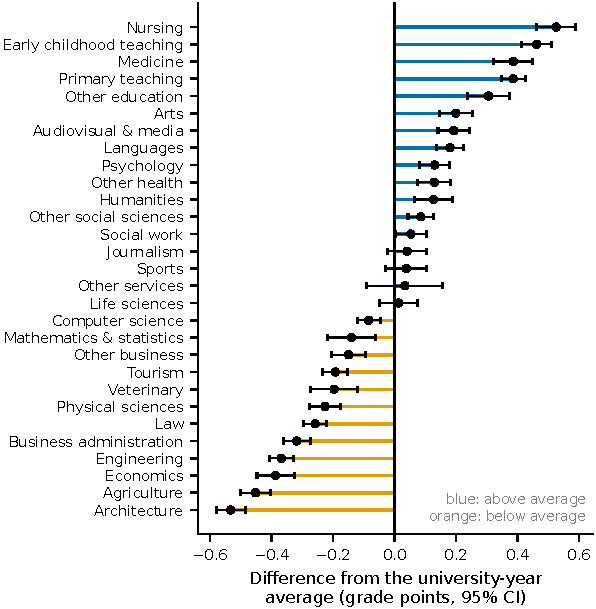
\includegraphics[width=\linewidth]{fig1_field_effects}
  \caption{\capguide{Ignacio -- see CAPTIONS.md, entry "Figure 1" (file fig1): what is shown (each field's distance from the average of all fields in the same university and year), data (SIIU, 12,125 means, 89 universities, 2015--16 to 2023--24, 5--10 scale), 95\% intervals clustered by university, colour meaning, source of the data.}}
  \label{fig:field-effects}
\end{figure}

We find the same broad ordering of components with the mixed model. Its descriptive comparison assigns approximately 61\% to the shared field pattern, 29\% to university-specific field differences and 11\% to the residual, compared with 65\%, 28\% and 7\% from nested least squares. The rounded mixed-model percentages need not sum to 100\%. The estimated variances are $\sigma_a^2=0.027$, $\sigma_b^2=0.039$ and $\sigma^2=0.015$ squared grade points, and the REML fit converged with L-BFGS. The interaction variance exceeds the residual variance, supporting a university profile beyond unexplained annual fluctuations. This does not establish persistence by itself; we test that interpretation on later years in Section~\ref{sec:res-prediction}. The two percentage splits are not identical estimands: one uses reductions in residual sums of squares after university-year adjustment, while the other combines fitted fixed-field variation with estimated interaction and residual variances. We saved the partially pooled profiles and conditional uncertainty intervals in \texttt{results/mixed\_model\_profiles.csv}, so the comparison need not rely on raw university averages alone.

% ============================================================
% 4.2 PERSISTENCE AND PREDICTION -- Writer: Ignacio Gimeno -- about 460 words
% THIS IS THE CORE ML RESULT AND THE ANSWER TO IDRIS ("what the model is,
% errors, tuning"). Every model in Table~\ref{tab:models} must be discussed, including what
% the tuning curves (Figure~\ref{fig:tuning}, file fig8_model_tuning) say.
% Numbers: results/progress_stats.json (persistence), results/model_selection_stats.json,
% results/model_selection_tuning.csv, results/final_figures_stats.json (fig2, fig8),
% figures/final/CAPTIONS.md (entries fig2 and fig8). Outline entries 6b and 6c.
% ============================================================

\subsection{University Profiles Persist and Predict Unseen Years}
\label{sec:res-prediction}

\guide{Ignacio -- Paragraph: persistence (Figure~\ref{fig:persistence})}{%
\textbf{Claim (outline 6b):} the university-specific part is stable over time.\\
\textbf{Numbers:} correlation between a field's university-specific deviation in consecutive years $r = 0.84$ (95\% CI 0.84--0.85), 10,413 pairs; least-squares slope 0.85, close to the dashed line of perfect persistence.\\
\textbf{Interpretation:} a stable pattern is what makes prediction possible, and also what makes a correction based on past years usable (\S\ref{sec:res-adjusted}).}
\budget{100}{Ignacio}

\begin{figure}[t]
  \centering
  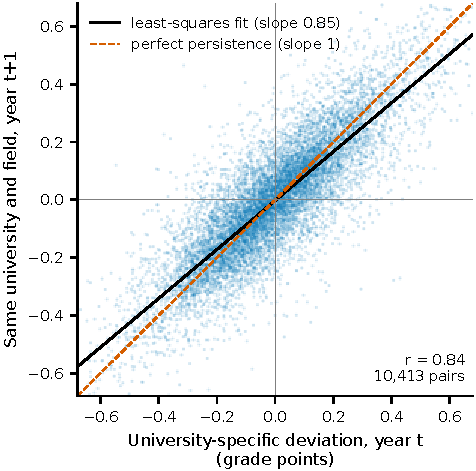
\includegraphics[width=0.92\linewidth]{fig2_persistence}
  \caption{\capguide{Ignacio -- see CAPTIONS.md, entry "Figure 2" (file fig2): what each point is (one university and field, two consecutive years), $r$ and number of pairs, meaning of the black and dashed red lines, units.}}
  \label{fig:persistence}
\end{figure}

\guide{Ignacio -- Paragraph: test errors (Table~\ref{tab:models})}{%
\textbf{Claim (outline 6c):} the university's own past is the best predictor of unseen years.\\
\textbf{Numbers (test 2022--2023):} baseline 0.365; common field effect 0.225; shrunk profile 0.138 (95\% CI 0.128--0.149); ridge 0.138; boosting 0.133. University profiles cut the error by 39\% relative to the shared effect; the paired bootstrap difference is $-0.098$ to $-0.077$ points, so the improvement is clear. $R^2$ rises from 0.62 to 0.86.\\
\textbf{Interpretation:} the 28\% university-specific share in \S\ref{sec:res-field} is real signal, not noise, because it predicts years the models never saw.}
\budget{130}{Ignacio}

% Table 2 -- prediction models. Numbers from results/model_selection_stats.json
% and results/model_selection_tuning.csv (checked 20 Nov 2026). Rounded to 3 d.p.
% Full grids: k in {0, 0.25, 0.5, 1, 2, 3, 5, 8, 13, 21, 50, inf}; alpha: 16
% log-spaced values from 1e-2 to 1e3; boosting: depth {2,3,5,8} x learning rate
% {0.03, 0.1, 0.3} x trees {100, 300, 600}.
\begin{table*}[t]
\centering
\caption{Prediction of a field's deviation from its university-year average, $d_{ufy}$, in grade points. Models are trained on 2015--2021, tuned by expanding-window validation on 2018--2021 (Algorithm~\ref{alg:tuning}; grids in \S\ref{sec:methods-prediction}) and evaluated once on 2022--2023 (2,774 university-field-years, 87 universities). The 95\% intervals come from 1,000 bootstrap resamples of universities. Lower RMSE and MAE are better.}
\label{tab:models}
\footnotesize
\setlength{\tabcolsep}{3.5pt}
\begin{tabular}{@{}lllcccc@{}}
\toprule
Model & Grid searched & Chosen & Valid.\ RMSE & Test RMSE (95\% CI) & Test MAE & Test $R^2$ \\
 & & & 2018--2021 & 2022--2023 & & \\
\midrule
Baseline (predict 0) & -- & -- & 0.360 & 0.365 (0.348--0.381) & 0.296 & 0.00 \\
Common field effect & -- & -- & 0.219 & 0.225 (0.211--0.241) & 0.174 & 0.62 \\
Shrunk university profile & 12 values, 0 to $\infty$ & $k = 0.25$ & 0.116 & 0.138 (0.128--0.149) & 0.103 & 0.86 \\
Ridge (field, university$\times$field) & 16 values, $10^{-2}$ to $10^{3}$ & $\alpha = 0.22$ & 0.116 & 0.138 (0.129--0.149) & 0.103 & 0.86 \\
Gradient boosting & 36 (depth, rate, trees) & 8, 0.03, 600 & 0.114 & 0.133 (0.123--0.143) & 0.098 & 0.87 \\
\bottomrule
\end{tabular}
\end{table*}


\guide{Ignacio -- Paragraph: what tuning shows (Figure~\ref{fig:tuning})}{%
\textbf{(a) Shrinkage:} the best $k$ is small (0.25): with up to seven past years, the university's own history deserves almost full weight; as $k$ grows the error rises towards the shared-effect line, which is the case $k=\infty$.\\
\textbf{(b) Ridge:} chosen $\alpha = 0.22$; same error as the shrunk profile (0.138) because both are forms of partial pooling -- a useful check that the result does not depend on one implementation. Large $\alpha$ removes the university terms and the error climbs.\\
\textbf{(c) Boosting:} the curve is almost flat (validation 0.116 at depth 2, 0.114 at depth 8); the chosen model (depth 8, rate 0.03, 600 trees) is at the edge of the grid, but the flat curve shows that larger models would gain little.}
\budget{130}{Ignacio}

\begin{figure*}[t]
  \centering
  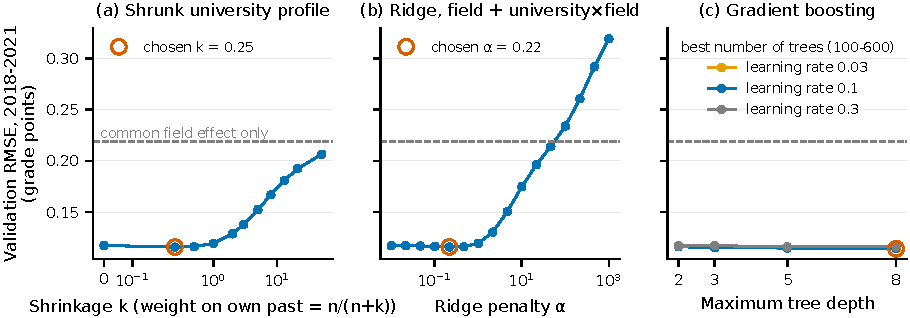
\includegraphics[width=\textwidth]{fig8_model_tuning}
  \caption{\capguide{Ignacio -- see CAPTIONS.md, entry "Figure 8" (file fig8): expanding-window validation error (2018--2021, grade points) for each value of the tuned hyperparameter; the red circle is the chosen value; dashed grey line = common field effect only; test years never used.}}
  \label{fig:tuning}
\end{figure*}

\guide{Ignacio -- Paragraph: which model we keep and why}{%
\textbf{Decision:} boosting is better than the shrunk profile by only 0.002--0.008 points (paired bootstrap, about 3\%), while the shrunk profile has one parameter and a direct reading (weight $n/(n+k)$ on the university's own past). We keep the shrunk profile for interpretation and for the adjusted mark. Boosting can also use dropout and size, yet it improves only slightly; do not claim more than that (no separate test removed those two features).\\
\textbf{Link:} the same idea -- use a university's past deviation -- is what makes the adjusted mark in \S\ref{sec:res-adjusted} work.}
\budget{100}{Ignacio}

\subsection{Student Intake Explains Little of the Field Differences}
\label{sec:res-confounders}

We find little evidence that the available intake measures account for the shared field pattern. Across 29 fields, the association between national admission grade and the field effect has slope 0.05 ($p=0.26$). In Figure~\ref{fig:confounders}, the points remain close to the no-change line when we add admission grade and size: before and after effects correlate 0.99, and their spread remains about 0.31 grade points. The figure covers 8,043 observations from 47 public universities. However, admission grades distinguish only five broad branches for 29 fields; they cannot separate intake within a branch, so the near-identity partly reflects this weak measurement. In the nested control analysis, the admission coefficient is 0.056 points per standard deviation ($p<0.001$), suggesting a small positive intake association without explaining away the field pattern.

\begin{figure}[t]
  \centering
  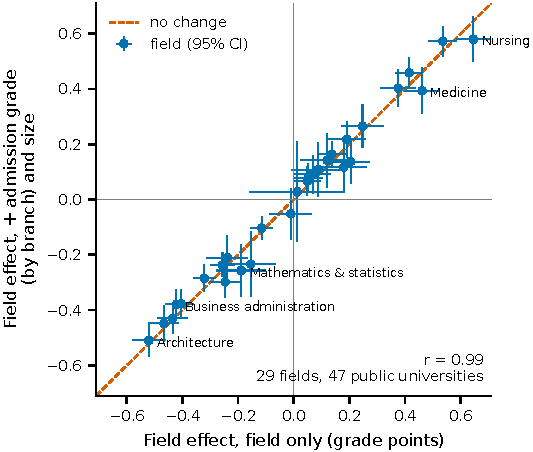
\includegraphics[width=0.92\linewidth]{fig3_confounders}
  \caption{Field effects before (horizontal axis) and after (vertical axis) adjustment for admission grade and size, in grade points on the Spanish 5--10 scale; SIIU, 8,043 records from 47 public universities. Bars show 95\% confidence intervals clustered by university; the dashed red line denotes no change. Admission grades identify only five broad branches, limiting adjustment within branches. Original figure; data from SIIU.}
  \label{fig:confounders}
\end{figure}

We obtained a similar conclusion using individual Portuguese entry grades. The gap between the highest- and lowest-graded degrees decreases from 1.51 to 1.30 points on the 0--20 scale after standardised entry grades and background controls. Degree remains jointly significant ($F=38.1$, 14 degrees of freedom, $p<0.001$). Most of the gap therefore remains even where intake is measured individually. We interpret this as an adjusted association, not evidence that equally able students would necessarily receive different grades if assigned to different degrees.

We found more attenuation when we added dropout: the spread falls from 0.31 to 0.24 points, and the effects correlate 0.95 with the original estimates. Higher dropout is associated with lower grades, but the direction is unresolved. Stricter grading may drive departures, while the remaining graduates are a selected group. We therefore report this specification separately rather than using it to claim that dropout causes the observed differences.

% ============================================================
% 4.4 SELECTION (first part) -- Writer: Ignacio Gimeno -- about 230 words
% Numbers: results/weighted_selection_by_field.csv, results/final_figures_stats.json
% (fig4), figures/final/CAPTIONS.md (entry fig4). Outline entries 8 [now 9] and 9a.
% Pablo's paragraph on the normal-approximation checks follows (04f).
% ============================================================

\subsection{A Single Raw-GPA Ranking Gives Unequal Access}
\label{sec:res-selection}

\guide{Ignacio -- Paragraph: Figure~\ref{fig:selection}}{%
\textbf{Claim (outline 9):} a single raw-GPA ranking gives very unequal access by field.\\
\textbf{Numbers:} in the median university-year, 41\% of Nursing graduates reach the top 20\% against 6\% of Business administration graduates (interquartile ranges 29--54\% and 2--13\%); 664 university-years, 79 universities.\\
\textbf{Must say (CAPTIONS.md):} these shares are simulated from published means and quartiles (\S\ref{sec:methods-simulation}), not observed selections.\\
\textbf{Interpretation:} with equal access every field would send 20\%; the field a student chose changes their chance of selection several times over.}
\budget{150}{Ignacio}

\begin{figure}[t]
  \centering
  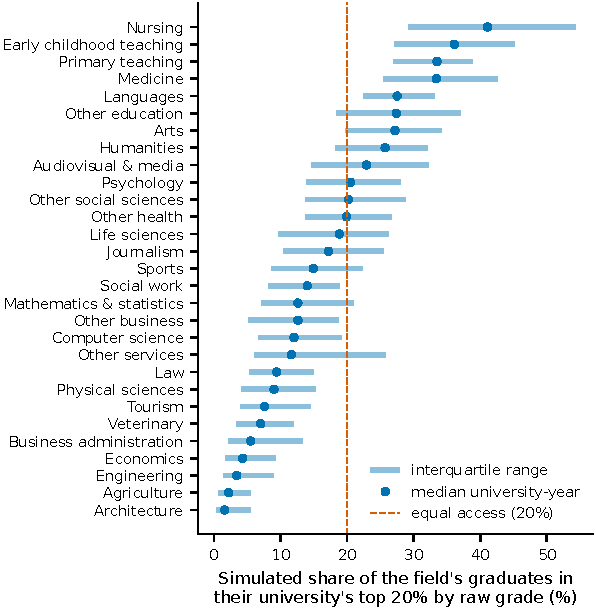
\includegraphics[width=\linewidth]{fig4_selection}
  \caption{\capguide{Ignacio -- see CAPTIONS.md, entry "Figure 4" (file fig4): simulated, not observed; normal approximation from mean and quartiles; graduate-weighted top-20\% cut per university-year; 664 university-years; median and interquartile range; dashed red line = equal access.}}
  \label{fig:selection}
\end{figure}

We find imperfections in the normal approximation but little sensitivity to truncation. Among 10,476 matched records, the median absolute mean--median gap is 0.11 estimated standard deviations and the median fitted probability outside 5--10 is about 0.04\%. The extreme tail fits less well: 23\% of available maxima lie outside their pointwise 95\% predictive intervals, and observed maxima exceed their expected values by 0.17 grade points on average. These discrepancies suggest that a normal distribution does not fully describe the upper tail; they are not formal evidence of a particular alternative distribution.

When we truncated the normal distributions to $[5,10]$, keeping the same underlying parameters and graduate weights, selection shares changed by a graduate-weighted average absolute difference of only 0.04 percentage points. The largest change in a field's average was 0.13 percentage points, and no field changed its overall rank. A pooled top-20\% threshold concerns the upper fifth rather than the single largest grade, explaining why imperfect maxima can coexist with stable selection estimates. We therefore regard Figure~\ref{fig:selection} as robust to this truncation check, without claiming robustness to every possible distribution or establishing normality from summaries.

% ============================================================
% 4.5 ADJUSTED MARKS -- Writer: Ignacio Gimeno -- about 320 words
% THIS ANSWERS IDRIS'S QUESTION: "Have you tried the suggestion in the previous
% feedback? and see if it makes GPA more equal?"  Answer it explicitly, with a
% real-life example (his Progress Report feedback asked for one).
% Numbers: results/adjusted_mark_stats.json, results/adjusted_mark_field_distribution.csv,
% results/final_figures_stats.json (fig7), figures/final/CAPTIONS.md (entry fig7).
% ============================================================

\subsection{Adjusted Marks Halve the Inequality}
\label{sec:res-adjusted}

\guide{Ignacio -- Paragraph: a worked example a reader can picture}{%
\textbf{Give one concrete case (Idris asked for a real-life result):} take a Nursing graduate and a Business administration graduate in the same university. Explain with the numbers of Figure~\ref{fig:field-effects} what their adjusted marks would be: on average Nursing grades sit $0.53$ points above the university-year average and Business administration $0.32$ below it (\texttt{results/final\_fig1\_field\_effects.csv}), so two students with the same raw mark, say 7.5, end up about $7.0$ and $7.8$ after adjustment -- 0.85 points apart, in favour of the Business student. In the method the deviation is the university's own past one, so the exact numbers vary by university; say that. Keep it simple and use the university's past deviation, as the method does.}
\budget{90}{Ignacio}

\guide{Ignacio -- Paragraph: the answer to Idris (Table~\ref{tab:adjusted}, Figure~\ref{fig:adjusted})}{%
\textbf{Claim:} yes -- the adjusted mark makes access much more equal, provided the deviation is estimated for each university.\\
\textbf{Numbers:} distance from equal access $G$: 11.8 pp with raw marks; 7.4 with the shared field deviation ($-37\%$); 5.1 with the university's average past deviation ($-57\%$), 95\% intervals 11.0--12.6 vs 4.8--5.3; upper bound with the same year's deviation 3.6 ($-69\%$). Nursing median 40.6\% $\to$ 13.0\%; Business administration 5.4\% $\to$ 19.5\%.\\
\textbf{Interpretation:} the ranking of the variants follows the prediction results in \S\ref{sec:res-prediction}: the better a correction predicts the deviation, the more equal the selection.}
\budget{120}{Ignacio}

% Table 3 -- adjusted marks. Numbers from results/adjusted_mark_stats.json
% (checked 20 Nov 2026). Evaluation 2016-2023, 595 university-years, 79 universities.
\begin{table}[t]
\centering
\caption{\capguide{Ignacio -- say: distance $G$ from equal access (equation~\eqref{eq:gap}), graduate-weighted, percentage points, 95\% interval from 1,000 bootstrap resamples of universities; medians across university-years for two fields; deviations estimated from earlier years except the last row (upper bound, not usable in practice); 2016--2023, 595 university-years.}}
\label{tab:adjusted}
\small
\setlength{\tabcolsep}{3.5pt}
\begin{tabularx}{\linewidth}{@{}>{\raggedright\arraybackslash}X c c c c@{}}
\toprule
Mark used for ranking & $G$ (pp) & 95\% CI & Nursing & Business \\
 & & & (\%) & adm.\ (\%) \\
\midrule
Raw mark & 11.8 & 11.0--12.6 & 40.6 & 5.4 \\
Minus shared field deviation & 7.4 & 7.1--7.7 & 14.4 & 17.7 \\
Minus university's deviation last year & 5.0 & 4.7--5.3 & 12.7 & 20.0 \\
Minus university's average past deviation & 5.1 & 4.8--5.3 & 13.0 & 19.5 \\
Minus same-year deviation (bound) & 3.6 & 3.4--3.8 & 12.8 & 20.5 \\
\bottomrule
\end{tabularx}
\end{table}


\begin{figure}[t]
  \centering
  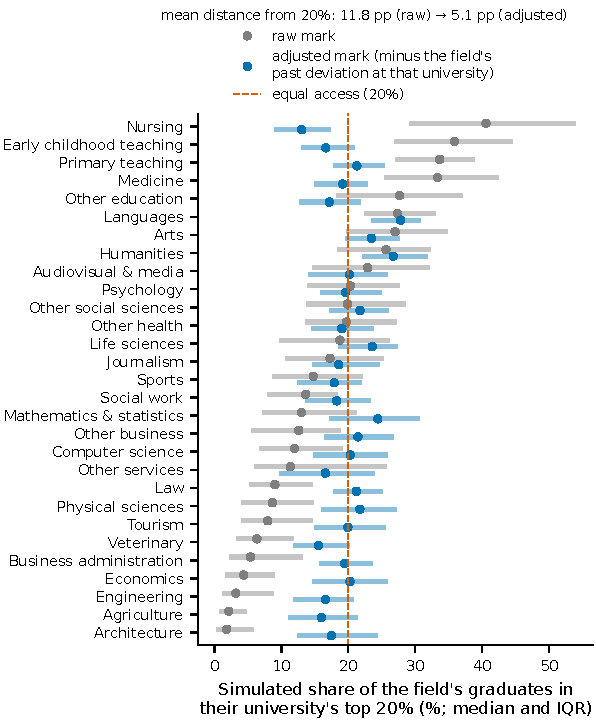
\includegraphics[width=\linewidth]{fig7_adjusted_marks}
  \caption{\capguide{Ignacio -- see CAPTIONS.md, entry "Figure 7" (file fig7): Figure~\ref{fig:selection} repeated with adjusted marks (minus the field's average past deviation at that university); median and interquartile range; 2016--2023, 595 university-years, so raw values differ slightly from Figure~\ref{fig:selection}; dashed line = equal access.}}
  \label{fig:adjusted}
\end{figure}

\guide{Ignacio -- Paragraph: why the adjusted mark is not enough on its own}{%
\textbf{Observation:} even with the same-year deviation (field means made equal), the median Nursing share is 12.8\% while Languages (27.8\%), Humanities (26.8\%) and Mathematics \& statistics (25.0\%) stay above 20\% (\texttt{adjusted\_mark\_field\_distribution.csv}, method \texttt{oracle\_current}). Equal means do not give equal access because fields differ in the \emph{spread} of their grades: a field with a narrow spread has few graduates in the upper tail. Evidence: median within-field standard deviation 0.44 points for Nursing (the narrowest) against 0.84 for Humanities and 0.87 for Languages (the widest) (\texttt{adjusted\_mark\_by\_field.csv}, column \texttt{median\_within\_field\_sd}).\\
\textbf{Consequence:} a correction must remove differences in spread as well as in level -- which is what ranking within the degree does (\S\ref{sec:res-rules}).\\
\textbf{Also say:} the 2016--2023 sample differs from Figure~\ref{fig:selection}, so the raw medians differ slightly (Nursing 40.6\% here, 41.1\% there).}
\budget{110}{Ignacio}

\subsection{Ranking Within the Degree Equalises Access with a Small Observed Grade Difference}
\label{sec:res-rules}

Ranking students within their degrees makes their chances of selection much more similar. Among the 3,469 students with grades in both semesters, the last panel of Figure~\ref{fig:rules} shows the standard deviation of selection rates falling from 0.090 under raw GPA (95\% interval 0.082--0.107) to 0.006 under percentiles (0.005--0.013). Regression adjustment and within-degree $z$-scores fall between them, at 0.040 and 0.019. The earlier exercise with all 3,703 students illustrates what this means: selection rates range from 5\% to 36\% under raw grades, compared with 19\% to 21\% under percentiles. In that larger sample, the within-degree rules change 138--156 of the 741 places.

\begin{figure*}[t]
  \centering
  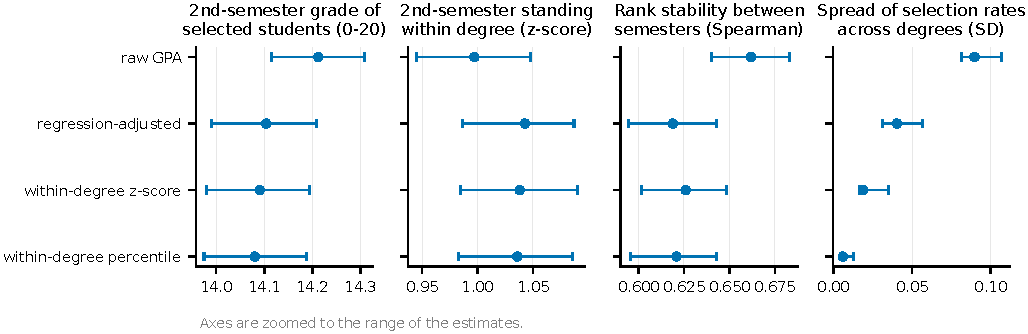
\includegraphics[width=\textwidth]{fig6_ranking_rules}
  \caption{Four rules selecting the top 20\% of 3,469 Portuguese students using first-semester grades, evaluated against second-semester outcomes, entry profile and selection balance. Bars show 95\% intervals from 1,000 student bootstrap resamples. Grade points use the 0--20 scale; standardised measures use standard-deviation units, and selection rates are proportions. Axes are zoomed: the raw-grade difference in the first panel is 0.13 points. Original figure; records from Realinho et al.}
  \label{fig:rules}
\end{figure*}

The difference in later grades is much smaller. Students selected by raw GPA average 14.21 in the second semester (14.11--14.31), compared with 14.08 under percentiles (13.97--14.19). That is a gap of 0.13 points on a 0--20 scale. The intervals overlap, although this alone does not prove that the rules perform equally or test the difference between them. If we look instead at students' standing within their degrees, the percentile rule comes out slightly ahead: the average standardised second-semester grade is 1.04, compared with 1.00 under raw GPA. Which result matters more depends on whether we want to reward reported grades or performance relative to classmates. Neither measure independently tells us how much students have learnt.

Raw GPA produces a more stable ranking between semesters, with a correlation of 0.66 compared with 0.62 for percentiles. However, grade differences between degrees can repeat too, contributing to that stability. A stable ranking is therefore not necessarily a more accurate measure of individual achievement. The selected students' mean standardised admission grades are 0.55 under raw GPA and 0.48 under percentiles, with overlapping intervals of 0.46--0.63 and 0.39--0.56. In this institution, percentiles give students much more similar chances across degrees, while the selected groups have broadly similar entry profiles and later grades.

% Adam report draft; prepared with AI assistance for author review.
\subsection{The US Data Show a Similar but Not Conclusive Pattern}
\label{sec:res-us}

The US results show moderate agreement with the Spanish pattern, although the evidence is not conclusive. Across ten comparable areas, Pearson correlation is $r=0.61$, with a 95\% Fisher-$z$ interval from $-0.03$ to $0.90$. Spearman correlation is also 0.61, and eight areas share the same sign. In Figure~\ref{fig:us}, Education has the highest effect in both countries: $+0.45$ Spanish grade points and $+0.43$ US GPA points. Engineering and Agriculture are below the centred reference in both. Adding area effects to university and year effects raises $R^2$ from 0.28 to 0.77 in the US and from 0.26 to 0.70 in Spain. This describes differences between aggregated cells. With only ten area pairs, the correlation remains uncertain: its interval includes zero, so the apparent agreement should be treated cautiously.

\begin{figure}[t]
  \centering
  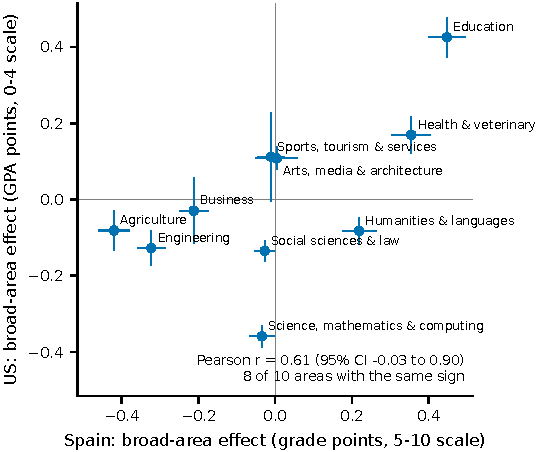
\includegraphics[width=0.92\linewidth]{fig5_us_spain}
  \caption{Fixed-effect estimates for ten common areas: Spanish graduate averages (5--10 scale) against US section GPAs (A+ = 4.3 conversion). Bars show 95\% intervals clustered by university. Pearson $r=0.61$ (95\% interval $-0.03$ to $0.90$); eight signs agree. Compare signs and ordering, not absolute magnitudes. Original figure; SIIU and Jeong et al.\ (``Course Grades'').}
  \label{fig:us}
\end{figure}

The countries do not agree in every area. Humanities and languages is above the reference in Spain ($+0.22$) but below it in the US ($-0.08$). Sports, tourism and services also changes sign, from $-0.01$ to $+0.11$, although both estimates are small. Science, mathematics and computing is close to the reference in Spain ($-0.03$) and further below it in the US ($-0.36$). These differences may partly reflect what the records measure. US departmental grades include introductory courses taken by students from other degrees, while the Spanish data describe graduates' final averages. Grouping subjects into broad areas can also hide differences within them, so we should not read every disagreement as evidence of a different grading policy.

The main result changes little across our checks. Pearson correlation is 0.62 with equal section weights across all 33 institutions, 0.61 when A+ is capped at 4.0, and 0.63 using common years. Each check keeps eight matching signs; capped-grade Spearman correlation is 0.70. Leaving out each US university keeps Pearson correlation between 0.60 and 0.63. This suggests that one institution does not drive the result, but it does not remove the uncertainty. The sensitivity runs use conventional coefficient errors, whereas Figure~\ref{fig:us} uses university-clustered intervals. The small number of areas and different grade definitions remain limitations.

\subsection{Limitations}
\label{sec:res-limitations}

Our data place several limits on what we can conclude. The Spanish records give average grades for graduates in each university, field and year. They cannot show how individual students change position, and they leave out students who do not graduate. Around half of the possible cells are unpublished, with smaller fields under-represented. We therefore simulated selection shares from published means and quartiles rather than observing actual selections. The checks in \S\ref{sec:res-selection} help assess the normal approximation, but cannot replace individual records. Admission-grade controls are also limited: they cover public universities and five broad branches, so they cannot separate the intake of fields within the same branch. Similar coefficients after adjustment therefore do not rule out differences in who enters each degree.

The Portuguese data let us follow individual students, but only at one polytechnic and into the next semester, among those with grades in both semesters. The US data cover more institutions, but the comparison has only ten areas and different grade types and years. Higher grades may reflect stronger learning as well as more generous grading. Making access more equal across degrees does not, by itself, show that we have removed grading bias or measured students' ability more accurately.


% ============================================================
% 5. CONCLUSIONS AND FUTURE WORK
% ============================================================
\section{Conclusions and Future Work}
\label{sec:conclusion}
% Adam report draft; prepared with AI assistance for author review.
Our results show that field of study is closely related to reported grades, and that these differences can affect access when students are ranked together. Shared field effects explain 65\% of the variation in Spanish field means within university-years; this is not a percentage of individual students' grades. In our simulation, the median share reaching the top 20\% is 41\% for Nursing and 6\% for Business administration. In Portugal, within-degree percentiles reduce the spread of selection rates from 0.090 to 0.006, with a small difference in later grades: 14.21 versus 14.08. The instructor's adjusted mark reduces the graduate-weighted distance from equal access from 11.8 to 5.1 percentage points, although differences in spread remain. Using universities' past field profiles also lowers test prediction error from 0.225 to 0.138 grade points. The US results suggest a similar broad-area pattern, but remain uncertain.

For institutions aiming to give students comparable chances across degrees, within-degree percentiles are worth considering. They account for differences in both average grades and their spread, while subtracting a field deviation changes only the average. ECTS grade-distribution tables offer a related way to put grades in context, although they do not prescribe a selection rule (European Commission 39--41). Institutions still need to decide what their ranking should reward. Our results describe associations between fields and grades; they do not establish that grading bias causes the gaps.

The next step is to test these ideas closer to actual decisions. Records of students taking shared courses, ideally with common assessments, could help separate preparation from grading differences. Individual Spanish records would let us examine real rankings rather than simulated selection shares. Finally, an exchange-allocation pilot could compare selection rules using later academic performance and participation across degrees, with the criteria agreed beforehand. This would help assess both the access benefits and possible costs that one semester's grades cannot capture.


% ============================================================
% WORKS CITED (MLA) -- not counted in the 10-12 pages
% ============================================================
% ============================================================
% WORKS CITED (MLA 9th edition) -- maintained by Ignacio Gimeno
% The brief requires MLA ("Use MLA style; the assignment requirement takes
% precedence over the template's default bibliography style").
%
% Every entry below was checked on 20 or 22 November 2026 against its DOI record
% (Crossref), the JMLR page (scikit-learn), the EU Publications Office page
% (ECTS guide), the Kaggle page (US dataset) or, for the Ministry tables, the
% Progress Report list. Do NOT add an entry you have not checked yourself.
%
% RULES
% - MLA lists ONLY works cited in the text. Before submission, delete every
%   entry that is not cited (each entry says where it is expected to be cited).
% - Alphabetical order by first author's surname; hanging indent; "---." when
%   the same author(s) as the entry above.
% - In-text format: (Achen and Courant 80) with page when quoting or pointing to
%   a specific claim, otherwise (Achen and Courant); three or more authors:
%   (Jeong et al.); two works by the same authors: add a short title, e.g.
%   (Jeong et al., "Construction") and (Jeong et al., "Course Grades");
%   Ministry tables: (Ministerio de Ciencia, Innovaci\'on y Universidades, "Media").
% ============================================================

\BAMunnumberedsection{Works Cited}
\label{sec:works-cited}
\begin{list}{}{\setlength{\leftmargin}{1.5em}\setlength{\itemindent}{-1.5em}\setlength{\itemsep}{0.25em}\setlength{\parsep}{0pt}}
\small
% cite in: Introduction 1.2 (grading differs by department)
\item Achen, Alexandra C., and Paul N. Courant. ``What Are Grades Made Of?'' \textit{Journal of Economic Perspectives}, vol.~23, no.~3, 2009, pp.~77--92, \url{https://doi.org/10.1257/jep.23.3.77}.
% cite in: Introduction 1.1 (background and major choice) -- checked 22 Nov 2026
\item Altonji, Joseph G., et al. `Heterogeneity in Human Capital Investments: High School Curriculum, College Major, and Careers.'' \textit{Annual Review of Economics}, vol.~4, 2012, pp.~185--223, \url{https://doi.org/10.1146/annurev-economics-080511-110908}.
% cite in: Introduction 1.1 (ability sorting into majors) -- checked 22 Nov 2026
\item Arcidiacono, Peter. `Ability Sorting and the Returns to College Major.'' \textit{Journal of Econometrics}, vol.~121, nos.~1--2, 2004, pp.~343--75, \url{https://doi.org/10.1016/j.jeconom.2003.10.010}.
% cite in: Introduction 1.2 (GPA measures and later outcomes) -- read the abstract first; checked 22 Nov 2026
\item Bailey, Michael A., et al. `Grades and Incentives: Assessing Competing Grade Point Average Measures and Postgraduate Outcomes.'' \textit{Studies in Higher Education}, vol.~41, no.~9, 2016, pp.~1548--62, \url{https://doi.org/10.1080/03075079.2014.982528}.
% cite in: Introduction 1.2 (grading differs by department) -- read the abstract first
\item Bar, Talia, et al. ``Grade Information and Grade Inflation: The Cornell Experiment.'' \textit{Journal of Economic Perspectives}, vol.~23, no.~3, 2009, pp.~93--108, \url{https://doi.org/10.1257/jep.23.3.93}.
% cite in: Methods 3.6 (expanding-window validation)
\item Bergmeir, Christoph, and Jos\'e M. Ben\'itez. ``On the Use of Cross-Validation for Time Series Predictor Evaluation.'' \textit{Information Sciences}, vol.~191, 2012, pp.~192--213, \url{https://doi.org/10.1016/j.ins.2011.12.028}.
% cite in: Introduction 1.2 (Wellesley grading policy) -- checked 22 Nov 2026
\item Butcher, Kristin F., et al. `The Effects of an Anti-Grade-Inflation Policy at Wellesley College.'' \textit{Journal of Economic Perspectives}, vol.~28, no.~3, 2014, pp.~189--204, \url{https://doi.org/10.1257/jep.28.3.189}.
% cite in: Methods 3.5 (clustered standard errors)
\item Cameron, A. Colin, and Douglas L. Miller. ``A Practitioner's Guide to Cluster-Robust Inference.'' \textit{Journal of Human Resources}, vol.~50, no.~2, 2015, pp.~317--72, \url{https://doi.org/10.3368/jhr.50.2.317}.
% cite in: Methods 3.5 (bootstrap)
\item Efron, Bradley. ``Bootstrap Methods: Another Look at the Jackknife.'' \textit{The Annals of Statistics}, vol.~7, no.~1, 1979, pp.~1--26, \url{https://doi.org/10.1214/aos/1176344552}.
% cite in: Methods 3.6 (shrinkage)
\item Efron, Bradley, and Carl Morris. ``Data Analysis Using Stein's Estimator and Its Generalizations.'' \textit{Journal of the American Statistical Association}, vol.~70, no.~350, 1975, pp.~311--19, \url{https://doi.org/10.1080/01621459.1975.10479864}.
% cite in: Introduction 1.2 (grade distribution tables) and Conclusions
\item European Commission. \textit{ECTS Users' Guide 2015}. Publications Office of the European Union, 2015, \url{https://doi.org/10.2766/87192}.
% cite in: Methods 3.6 (gradient boosting)
\item Friedman, Jerome H. ``Greedy Function Approximation: A Gradient Boosting Machine.'' \textit{The Annals of Statistics}, vol.~29, no.~5, 2001, pp.~1189--232, \url{https://doi.org/10.1214/aos/1013203451}.
% cite in: Appendix (software)
\item Harris, Charles R., et al. ``Array Programming with NumPy.'' \textit{Nature}, vol.~585, no.~7825, 2020, pp.~357--62, \url{https://doi.org/10.1038/s41586-020-2649-2}.
% cite in: Methods 3.6 (ridge)
\item Hoerl, Arthur E., and Robert W. Kennard. ``Ridge Regression: Biased Estimation for Nonorthogonal Problems.'' \textit{Technometrics}, vol.~12, no.~1, 1970, pp.~55--67, \url{https://doi.org/10.1080/00401706.1970.10488634}.
% cite in: Appendix (software)
\item Hunter, John D. ``Matplotlib: A 2D Graphics Environment.'' \textit{Computing in Science \& Engineering}, vol.~9, no.~3, 2007, pp.~90--95, \url{https://doi.org/10.1109/MCSE.2007.55}.
% cite in: Introduction, Data 2.3, Methods 3.9, Results 4.7
\item Jeong, Hyun, et al. ``The Construction and Analysis of Course Grades Across Public Universities.'' \textit{Proceedings of the 17th International Conference on Educational Data Mining}, 2024, pp.~643--48, \url{https://doi.org/10.5281/zenodo.12729906}.
% cite in: Data 2.3 -- Adam: replace the access date with the day you downloaded the files
\item ---. ``Course Grades from 33 Public Universities.'' \textit{Kaggle}, \url{https://www.kaggle.com/datasets/hyunjeong2023/edm-grading-dataset}. Accessed 9 Nov. 2026.
% cite in: Introduction 1.2 (adjusted GPA) -- checked 22 Nov 2026
\item Johnson, Valen E. `An Alternative to Traditional GPA for Evaluating Student Performance.'' \textit{Statistical Science}, vol.~12, no.~4, 1997, pp.~251--78, \url{https://doi.org/10.1214/ss/1030037959}.
% cite in: Introduction 1.1 (family background and major choice) -- checked 22 Nov 2026
\item Ma, Yingyi. `Family Socioeconomic Status, Parental Involvement, and College Major Choices---Gender, Race/Ethnic, and Nativity Patterns.'' \textit{Sociological Perspectives}, vol.~52, no.~2, 2009, pp.~211--34, \url{https://doi.org/10.1525/sop.2009.52.2.211}.
% cite in: Appendix (software)
\item McKinney, Wes. ``Data Structures for Statistical Computing in Python.'' \textit{Proceedings of the 9th Python in Science Conference}, 2010, pp.~56--61, \url{https://doi.org/10.25080/Majora-92bf1922-00a}.
% cite in: Data 2.1 (graduates per field)
\item Ministerio de Ciencia, Innovaci\'on y Universidades. ``Egresados por sexo, grupo de edad y \'ambito de estudio.'' \textit{Estad\'istica de Estudiantes Universitarios}, Sistema Integrado de Informaci\'on Universitaria (SIIU), 2025, \url{https://estadisticas.ciencia.gob.es}. Accessed 24 Oct. 2026.
% cite in: Data 2.1 (main grade table)
\item ---. ``Media, cuartiles y m\'aximo de la nota del expediente (estudiantes egresados) por \'ambito de estudio y sexo.'' \textit{Sistema Integrado de Informaci\'on Universitaria (SIIU)}, 2025, \url{https://estadisticas.ciencia.gob.es}. Accessed 10 Oct. 2026.
% cite in: Data 2.1 (admission grade by branch)
\item ---. ``Nota media y cuartiles de nota de admisi\'on de los estudiantes de nuevo ingreso en Grado por forma de admisi\'on, sexo y rama de ense\~nanza.'' \textit{Estad\'istica de Estudiantes Universitarios}, Sistema Integrado de Informaci\'on Universitaria (SIIU), 2025, \url{https://estadisticas.ciencia.gob.es}. Accessed 24 Oct. 2026.
% cite in: Data 2.1 (national admission grade by field)
\item ---. ``Nota media y cuartiles de nota de admisi\'on de los estudiantes de nuevo ingreso en Grado por forma de admisi\'on, sexo y \'ambito de estudio.'' \textit{Estad\'istica de Estudiantes Universitarios}, Sistema Integrado de Informaci\'on Universitaria (SIIU), 2025, \url{https://estadisticas.ciencia.gob.es}. Accessed 24 Oct. 2026.
% cite in: Data 2.1 (dropout)
\item ---. ``Tasas de abandono del estudio (cohortes de nuevo ingreso en el estudio) por \'ambito de estudio y sexo.'' \textit{Sistema Integrado de Informaci\'on Universitaria (SIIU)}, 2025, \url{https://estadisticas.ciencia.gob.es}. Accessed 24 Oct. 2026.
% cite in: Introduction 1.2 (grades and persistence in science) -- checked 22 Nov 2026
\item Ost, Ben. `The Role of Peers and Grades in Determining Major Persistence in the Sciences.'' \textit{Economics of Education Review}, vol.~29, no.~6, 2010, pp.~923--34, \url{https://doi.org/10.1016/j.econedurev.2010.06.011}.
% cite in: Appendix (software)
\item Pedregosa, Fabian, et al. ``Scikit-learn: Machine Learning in Python.'' \textit{Journal of Machine Learning Research}, vol.~12, 2011, pp.~2825--30.
% cite in: Introduction 1.2 (grades and attrition from STEM) -- checked 22 Nov 2026
\item Rask, Kevin. `Attrition in STEM Fields at a Liberal Arts College: The Importance of Grades and Pre-Collegiate Preferences.'' \textit{Economics of Education Review}, vol.~29, no.~6, 2010, pp.~892--900, \url{https://doi.org/10.1016/j.econedurev.2010.06.013}.
% cite in: Data 2.2 (dataset)
\item Realinho, Valentim, et al. ``Predict Students' Dropout and Academic Success.'' \textit{UCI Machine Learning Repository}, 2021, \url{https://doi.org/10.24432/C5MC89}.
% cite in: Data 2.2 (description of the dataset) -- optional
\item ---. ``Predicting Student Dropout and Academic Success.'' \textit{Data}, vol.~7, no.~11, 2022, p.~146, \url{https://doi.org/10.3390/data7110146}.
% cite in: Introduction 1.2 (grading differs by department)
\item Sabot, Richard, and John Wakeman-Linn. ``Grade Inflation and Course Choice.'' \textit{Journal of Economic Perspectives}, vol.~5, no.~1, 1991, pp.~159--70, \url{https://doi.org/10.1257/jep.5.1.159}.
% cite in: Methods 3.2 and Appendix (software)
\item Seabold, Skipper, and Josef Perktold. ``Statsmodels: Econometric and Statistical Modeling with Python.'' \textit{Proceedings of the 9th Python in Science Conference}, 2010, pp.~92--96, \url{https://doi.org/10.25080/Majora-92bf1922-011}.
% cite in: Appendix (software)
\item Virtanen, Pauli, et al. ``SciPy 1.0: Fundamental Algorithms for Scientific Computing in Python.'' \textit{Nature Methods}, vol.~17, no.~3, 2020, pp.~261--72, \url{https://doi.org/10.1038/s41592-019-0686-2}.
% cite in: Introduction 1.2 (adjusted GPA with item response theory) -- checked 22 Nov 2026
\item Young, John W. `Adjusting the Cumulative GPA Using Item Response Theory.'' \textit{Journal of Educational Measurement}, vol.~27, no.~2, 1990, pp.~175--86, \url{https://doi.org/10.1111/j.1745-3984.1990.tb00741.x}.
% cite in: Introduction 1.1 (gender gap in major choice) -- checked 22 Nov 2026
\item Zafar, Basit. `College Major Choice and the Gender Gap.'' \textit{Journal of Human Resources}, vol.~48, no.~3, 2013, pp.~545--95, \url{https://doi.org/10.3368/jhr.48.3.545}.
\end{list}


% ============================================================
% DECLARATION OF CONTRIBUTIONS
% ============================================================
\BAMunnumberedsection{Declaration of Contributions}
\label{sec:contributions}
% ============================================================
% DECLARATION -- Teamwork and Review Process -- Writer: Ignacio Gimeno
% Template: "Explain how work was coordinated, how members reviewed or tested
% one another's contributions, how disagreements or changes were handled, and
% how the team approved the final submission. Do not imply equal contributions
% unless they were genuinely equal."
% Brief: "Students must be able to connect the repository history to the
% submitted analysis."
% ============================================================

\subsection*{Teamwork and Review Process}

\guide{Ignacio -- Teamwork and review (about 120 words)}{%
\textbf{Facts you can state (all visible in the repository):} work organised through GitHub issues, one branch per task and pull requests reviewed by another member before merging (PRs \#5--\#10 and the report PRs); each member reran another member's code and checked that the saved results reproduce (for example the independent reproduction of the US results and of the mixed model); the report was written section by section from the agreed Sentence Outline, each member writing their own sections; the team read and approved the final version before submission.\\
\textbf{Material changes from the plan:} after the Sentence Outline feedback the team added the adjusted-mark analysis and the tuned model comparison.\\
\textbf{Repository:} \url{https://github.com/ngimenoieu2025-lang/FIELD-GPA-Ranking} (give the final commit in the Appendix).}
\budget{120}{Ignacio}


\subsection*{Individual Contributions}
\subsubsection*{Adam Bajer}
I contributed the US replication scripts, department mappings, tests, comparison figure and findings through the US replication pull request. My assigned sections cover fairness, US data and methods, computing, ranking-rule and US results, limitations, conclusions and reproducibility. Checks included six passing tests and reproduction of the saved Spanish coefficients. Ignacio independently reproduced the US results.

% ============================================================
% DECLARATION -- Individual contribution -- Writer: Pablo Torres
% Template: identify concrete contributions and the outputs or decisions for
% which the member was responsible. Start from your Sentence Outline entry.
% ============================================================

\subsubsection*{Pablo Torres}
\guide{Pablo -- Your contribution (about 70 words)}{%
Concrete outputs: mixed-effects model (\texttt{src/mixed\_model.py}, \texttt{results/mixed\_model\_*}), normal-approximation checks and truncated-normal sensitivity (\texttt{src/normal\_check.py}); report sections 2 (Data), 3.1--3.5 and the mixed-model and normal-check paragraphs of Section 4; Table~\ref{tab:data} caption; review of pull requests. Name the decisions you made (for example REML, the truncation check).}
\budget{70}{Pablo}

% ============================================================
% DECLARATION -- Individual contribution -- Writer: Ignacio Gimeno
% ============================================================

\subsubsection*{Ignacio Gimeno}
Ignacio found the Spanish Ministry and Portuguese data, proposed the research question and carried out the Spanish analysis: the variance decomposition, persistence, temporal validation, confounder controls and selection simulation. After the Sentence Outline feedback, he added the adjusted-mark analysis, the tuned comparison of prediction models and the analysis of student background. He also compared the ranking rules, produced the final figures and organised the repository and README. In the report, he was responsible for Sections 1.1, 1.3, 3.6--3.8, 4.1, 4.2 and 4.5 and the abstract, and he integrated the sections, checked every number against the saved results and prepared the submission.


% ============================================================
% APPENDIX -- not counted in the 10-12 pages
% ============================================================
\BAMappendices
% ============================================================
% APPENDIX A -- CODE, DATA AND REPRODUCIBILITY -- Writer: Adam Bajer
% Not counted in the 10-12 pages. Template: "Repository URL; exact release,
% tag, or commit; ... software and versions; installation; data preparation;
% configuration; random seeds; execution commands; mapping from scripts or
% notebooks to results; hardware requirements; expected runtime; and known
% issues." Brief: the repository must be organised, readable and reproducible.
% The tables below are factual (checked on 20 Nov 2026); the prose is yours.
% ============================================================

\section{Code, Data, and Reproducibility}
\label{app:reproducibility}

Our code is at \url{https://github.com/ngimenoieu2025-lang/FIELD-GPA-Ranking}; final commit: \texttt{[insert after final merge]}. The README explains installation and execution. Ministry and UCI data are included; the US files require a separate download (about 274 MB). Tables~\ref{tab:software} and~\ref{tab:pipeline} give software versions and run order. Random seeds are 42. The recorded 22 November rerun took about 16 minutes, excluding the US replication. Saved tables and JSON results matched, apart from eighth-decimal differences in mixed-model shares. The libraries used were NumPy, pandas, SciPy, statsmodels, scikit-learn and Matplotlib (Harris et al.; McKinney; Virtanen et al.; Seabold and Perktold; Pedregosa et al.; Hunter).

\begin{table}[H]
\centering
\caption{Hardware and software used in the team's documented rerun on 22 November 2026. The versions describe that setup; they are not minimum requirements.}
\label{tab:software}
\small
\begin{tabularx}{\linewidth}{@{}l>{\raggedright\arraybackslash}X@{}}
\toprule
Component & Version \\
\midrule
Hardware & Intel Core Ultra 7 258V (8 cores), 32 GB RAM, no GPU \\
Operating system & Windows 11 (build 26200) \\
Python & 3.14.4 \\
NumPy & 2.4.4 \\
pandas & 3.0.2 \\
SciPy & 1.18.1 \\
statsmodels & 0.15.0 \\
scikit-learn & 1.9.1 \\
Matplotlib & 3.10.9 \\
\bottomrule
\end{tabularx}
\end{table}

\begin{table*}[t]
\centering
\caption{Scripts in run order, the outputs they produce and where those outputs appear in the report. Run scripts from the repository root with \texttt{python src/<script>}; install dependencies with \texttt{pip install -r requirements.txt}. Outputs are saved under \texttt{results/} and \texttt{figures/}. Times are from the documented 22 November run; -- denotes an unmeasured US runtime, excluded from the approximately 16-minute total.}
\label{tab:pipeline}
\footnotesize
\begin{tabularx}{\textwidth}{@{}l>{\raggedright\arraybackslash}X>{\raggedright\arraybackslash}Xr@{}}
\toprule
Script (\texttt{src/}) & Main outputs & Used in & Time \\
\midrule
\texttt{load\_data.py}, \texttt{analysis.py} & cleaned Portuguese records, degree effects & \S\ref{sec:data-portugal}, \S\ref{sec:res-confounders} & 33 s \\
\texttt{ministry.py}, \texttt{progress.py} & decomposition, persistence, confounders, selection shares & \S\ref{sec:res-field}--\S\ref{sec:res-selection}, Figures~\ref{fig:field-effects}--\ref{fig:selection} & 6.6 min \\
\texttt{mixed\_model.py} & variance components, university profiles & \S\ref{sec:res-field} & 27 s \\
\texttt{normal\_check.py} & normal-approximation diagnostics, truncated-normal selection & \S\ref{sec:res-selection} & 51 s \\
\texttt{ranking\_rules.py} & four ranking rules with bootstrap intervals & \S\ref{sec:res-rules}, Figure~\ref{fig:rules} & 3.3 min \\
\texttt{background.py} & background of the students of each degree & \S\ref{sec:context}, Figure~\ref{fig:background} & 3 s \\
\texttt{us\_replication.py} (+ \texttt{us\_mapping.py}, \texttt{us\_model.py}) & US cells, crosswalk, country comparison, sensitivity checks & \S\ref{sec:res-us}, Figure~\ref{fig:us} & -- \\
\texttt{adjusted\_mark.py} & adjusted-mark selection shares & \S\ref{sec:res-adjusted}, Table~\ref{tab:adjusted}, Figure~\ref{fig:adjusted} & 25 s \\
\texttt{model\_selection.py} & tuning curves, test errors & \S\ref{sec:res-prediction}, Table~\ref{tab:models}, Figure~\ref{fig:tuning} & 3.4 min \\
\texttt{final\_figures.py} (run last) & the nine data figures of this report, \texttt{final\_figures\_stats.json} & all figures & 25 s \\
\bottomrule
\end{tabularx}
\end{table*}


\end{document}
